% manuscript.tex -- Journal of Systems and Software submission.
% Special Issue "AI Techniques for Performance, Reliability, and
% Sustainability of Modern Software Systems" (VSI:AI4MSS).

\documentclass[preprint,3p]{elsarticle}

\usepackage[T1]{fontenc}
\usepackage{lmodern}
\usepackage{array}
\usepackage{calc}
\usepackage{amsmath,amssymb}
\usepackage{graphicx}
\usepackage{booktabs}
\usepackage{multirow}
\usepackage{longtable}
\usepackage{lineno}
\usepackage{xcolor}
\usepackage{textcomp}
\usepackage{xr-hyper}
\usepackage{hyperref}
\usepackage{microtype}

% Float packing: the default Elsevier preprint parameters strand large tables and
% leave partially-filled pages. These are typesetting settings only.
\renewcommand{\topfraction}{0.9}
\renewcommand{\bottomfraction}{0.8}
\renewcommand{\textfraction}{0.07}
\renewcommand{\floatpagefraction}{0.75}
\setcounter{topnumber}{3}
\setcounter{bottomnumber}{2}
\setcounter{totalnumber}{5}

\setlength{\textfloatsep}{7pt plus 2pt minus 2pt}
\setlength{\intextsep}{7pt plus 2pt minus 2pt}
\setlength{\floatsep}{6pt plus 2pt minus 2pt}
\setlength{\abovecaptionskip}{3pt}
\setlength{\belowcaptionskip}{1pt}

% Experiment pages in the public replication repository, pinned to the submission tag.
\newcommand{\sagexperimentsurl}{https://github.com/onuralpyigit/software-as-a-graph/tree/main/docs/research/jss/experiments}
\newcommand{\sagexperiments}{\url{\sagexperimentsurl}}

\providecommand{\tightlist}{%
  \setlength{\itemsep}{0pt}\setlength{\parskip}{0pt}}

\journal{Journal of Systems and Software}

\begin{document}

\begin{frontmatter}

\title{Software-as-a-Graph: Learning Cascade-Impact Rankings
  from Dependency Graphs of Publish--Subscribe Systems}

\author[itu]{Ibrahim Onuralp Yigit\corref{cor1}}
\ead{yigiti@itu.edu.tr}
\author[itu]{Feza Buzluca}
\ead{buzluca@itu.edu.tr}

\affiliation[itu]{organization={Department of Computer Engineering, Istanbul Technical University},
             city={Istanbul}, postcode={34469}, country={Turkey}}
\cortext[cor1]{Corresponding author}

\begin{abstract}
Publish--subscribe middleware is fundamental to modern distributed systems, but its decoupled topic abstractions frequently obscure cascading failure paths. To address this, Software-as-a-Graph (SaG) models event-driven systems as typed multigraphs and derives explicit dependency graphs from deployment manifests. This study evaluates learned cascade-impact rankers, including graph neural networks, hybrid engines, and learned surrogates, on twelve synthetic architectures using leave-one-scenario-out cross-validation, against three failure simulators, and zero-shot on five stylized models of open-source systems.

Deriving dependency graphs improves learned ranking: graph attention networks gain $+0.08$ to $+0.11$ over the raw multigraph, reaching a Spearman $\rho$ of $0.748$ against the reachability simulator. This is statistically indistinguishable from counting direct dependents ($0.764$), a classical coupling metric that restates the simulator's first propagation wave, and the match relies on degree features supplied to the networks. Learning pays off where simulation is costly. On a dynamic queue-flow simulator requiring $12.7$ CPU-hours to label the corpus, a gradient-boosted surrogate using dependency, rate, payload, and QoS features ranks held-out architectures above every closed-form approximation tested ($0.799$ vs.\ $0.706$; nominal $p = 0.019$), replacing hours of simulation with inference in seconds. Under multi-criteria fragmentation, hybrids retain accuracy through their closed-form prior ($\rho = 0.585$ vs.\ $\le 0.334$ without it). Pure learned models transfer best to unfamiliar systems ($\rho = 0.805$ vs.\ $0.662$--$0.695$ for hybrids), mainly by separating inert from active components; ranking within the active stratum remains challenging ($\rho_{>0} \le 0.342$). The results support a practical, energy-aware two-tier approach, conditional on simulator fidelity: instant dependency counting for commit-stage triage, and learned surrogates for verification during staging.

\end{abstract}

\begin{keyword}
Dependency graphs \sep
cascading failures \sep
publish--subscribe \sep
graph neural networks \sep
graph learning \sep
software architecture \sep
dependability \sep
empirical study
\end{keyword}

\end{frontmatter}

\linenumbers

\section{Introduction}
\label{sec:1}

\subsection{Motivation and Problem}
\label{sec:1.1}

Large distributed systems now often use asynchronous publish-subscribe (pub-sub) middleware. Examples include ROS 2 for autonomous driving \cite{macenski2022robot}, Apache Kafka for enterprise event streams \cite{kreps2011kafka}, DDS in cyber-physical systems \cite{omg2015dds}, MQTT in IoT \cite{oasis2019mqtt}, and cloud-native microservices \cite{dragoni2017microservices,newman2015building}. Pub-sub separates producers and consumers by space, time, and synchronization \cite{eugster2003faces}. Instead of direct references, components communicate via topics and brokers, and Quality-of-Service (QoS) policies set at deployment control reliability, durability, priority, and deadlines.

This decoupling also makes it harder to see how failures spread. Since publishers and subscribers are not directly connected, problems like outages, blocking, and backpressure can move through undetected paths involving brokers, shared topics, colocated hosts, and shared libraries \cite{motter2002cascade,buldyrev2010cascade}. Failures usually appear in two ways. In sequential cascades, a slow subscriber fills up a broker queue and gradually starves its publishers \cite{albert2000error}. In simultaneous blasts, a crash in a shared library or a host outage can bring down all colocated services at once. These issues are not visible in architecture diagrams or static call graphs. The best time to handle these risks is before deployment, during design and continuous integration \cite{avizienis2004basic,bass2012software}, when runtime telemetry is unavailable. Therefore, architects must identify the most critical components, topics, and links using only configuration manifests.

Current practices leave a serious gap, which we call the Architecture–Code Gap. A distributed system might have no compile-time bugs in any service but still face major outages due to hidden single points of failure, unbuffered queue bottlenecks, or mismatched QoS contracts \cite{perry1992foundations,garcia2009identifying}. Approaches like the Architecture Tradeoff Analysis Method (ATAM) depend on manual input \cite{kazman1998atam}. Static code analysis inspects services in isolation \cite{sonarsource2024clean,chidamber1994metrics}. Chaos engineering \cite{basiri2016chaos} needs a working cluster, and pre-production tests like fault injection \cite{meiklejohn2021service} and dependency tracing \cite{yu2021microrank} require runnable environments. In continuous integration, heavy fault injection or chaos experiments use significant computing power and energy, so pre-deployment static analysis is a greener option if it is accurate enough \cite{calero2015green,verdecchia2023greenai,schwartz2020greenai}. Homogeneous centrality reduces typed topologies to untyped graphs \cite{freeman1977centrality,brandes2001faster}. Graph neural networks can combine structural and contractual information, but only if the graph clearly shows failure paths. Software-as-a-Graph provides this representation, turning static deployment manifests into predictive insights before deployment and enabling a two-tier triage process to reduce developer alert fatigue.

\subsection{The Software-as-a-Graph (SaG) Approach}
\label{sec:1.3}

Software-as-a-Graph (SaG) is a static analysis framework used before deployment for event-driven architectures (see Figure~\ref{fig:1}). First, it models the architecture as a typed, directed multigraph that includes Applications, Brokers, Topics, Execution Hosts, and Shared Libraries (Section~\ref{sec:3.1}). Next, it uses publish-subscribe rules to create a clear DEPENDS\_ON dependency graph (Section~\ref{sec:3.3}). Then, it tests learned cascade-impact rankers—such as graph neural networks on both the raw multigraph and the dependency graph, hybrids, and learned surrogates—against a baseline that does not use training (Sections~\ref{sec:4} and~\ref{sec:6.2}). The predictors only use the analysis graph. Three simulators provide ground truth by running on the base structural topology (Section~\ref{sec:4.3}). To measure architectural risk without relying on single or unproven assumptions, SaG uses a tri-oracle evaluation suite. This suite covers structural reachability ($I^*$), dynamic discrete-event queue saturation ($I_{\text{dyn}}$), and multi-criteria service fragmentation ($I_{\text{comp}}$). The main reachability oracle $I^*$ works directly on communication topologies defined in the manifest, so its first-order propagation matches direct dependency counts (Section~\ref{sec:4.4}). To avoid mixing up structural alignment regarding predictive learning, the method tracks dependency counts as baseline references and carefully tests how well learned models generalize to dynamic queue flows and structural fragmentation. To bound, though not remove, this circularity, the evaluation uses three simulators with different mechanisms, reports partial correlations after removing the primary oracle, and times the cost of running $I^*$ directly (Section~\ref{sec:rq4}). Verifying these results against real-world failures is still an important goal (Section~\ref{sec:8.3}). The conclusions and guidance here are valid as long as the simulations are accurate.

\noindent\textbf{Findings in brief.} Making dependencies explicit is what enables graph learning in this setting. On the raw multigraph, every relation points away from Applications, so message passing never reaches the scored nodes. Accordingly, the registered primary contrast, a heterogeneous graph transformer against the training-free baseline on that graph, showed no significant difference ($\Delta\rho = +0.069$, $p = 0.266$). On the derived dependency graph, each Application receives messages from its dependents, and the same learners improve by $+0.08$ to $+0.11$. There, a graph attention network reaches Spearman $\rho = 0.748$ against the reachability oracle.
This matches the number of direct dependents ($0.764$) within statistical resolution. That count is publish--subscribe afferent coupling, which corresponds to the oracle's first propagation wave. Ablations explain the match: the learner draws on its degree features and loses $0.14$ when they are removed. The practical implication is a training-free triage signal for reachability impact that costs one to two orders of magnitude less than a single simulation pass.
Learning adds most where simulation is expensive. On a discrete-event queue-flow oracle that takes $12.7$ CPU-hours to label the corpus, a gradient-boosted surrogate combining dependency, rate, payload and QoS features ranks held-out architectures at $\rho = 0.799$. It outperforms every closed-form approximation tested ($0.706$; nominal $p = 0.019$) and replaces hours of simulation with inference in seconds. On this oracle, declared QoS contracts contribute measurable signal ($+0.095$).
On a multi-criteria oracle that combines fragmentation and throughput loss, hybrid engines that correct a closed-form prior remain accurate ($\rho = 0.585$), whereas learners without a prior degrade ($\rho \le 0.334$). As expected, training-free scores aligned with that oracle's terms rank higher still. Pure learned engines, in turn, transfer best zero-shot to five stylized models of open-source systems ($\rho \approx 0.81$ vs.\ $0.66$--$0.70$ for hybrids). They do so mainly by separating components that propagate failures from those that do not, with transitive-dependent counts ranking even higher. Ordering among active components remains the open challenge ($\rho_{>0} \le 0.342$).
These results translate into concrete guidance. Recovering 80\% of the true critical set requires reviewing roughly the top 40\% of Applications, so rankings are best used to prioritize architectural review rather than to block commits. Feature extraction costs $4.5$--$72.5\times$ one reachability pass, so dependency counting suits commit-stage triage, while learned surrogates suit staging, where they replace expensive simulation (Section~\ref{sec:8.1}). All findings are relative to simulated failures.

\subsection{Research Questions}
\label{sec:1.4}

\begin{itemize}\tightlist
\item \textbf{RQ1 (Ranking accuracy):} \emph{How accurately do learned engines rank components by cascading-failure impact on unseen architectures, against a training-free baseline, and how close do they come to reference rankings that restate the oracle’s propagation rule?}
\item \textbf{RQ2 (What learning needs):} \emph{What do learned engines need: which graph they read, their degree features, relation-specific parameters, or QoS inputs, once model capacity and edge-channel width are matched?}
\item \textbf{RQ3 (Transfer):} \emph{How well do learned engines trained using synthetic architectures transfer zero-shot to stylized architectural models hand-authored by a single modeler based on five open-source systems, and does within-cascade discrimination hold on the active stratum?}
\item \textbf{RQ4 (Cost and Sustainability):} \emph{What does learned ranking cost at CI/CD time with respect to latency and computational energy, which stage dominates, and how does it compare with running the simulation directly?}
\end{itemize}

The evaluation uses a version-controlled analysis plan. Only two contrasts in the plan are confirmatory. We registered the matched $2\times2$, the hybrids, the reference counts, the dependency-graph learners, the full-population queue-flow labels, and the sensitivity arms as planned extensions. We registered each before its own tests ran but after we knew the main result, and we report them as secondary results. The rest of the analysis is exploratory (Section~\ref{sec:6.3}). One change from the plan, an unused selection rule, is disclosed and tested. The replication repository records the revision history and shows how these four research questions fit into the plan.

\subsection{Contributions}
\label{sec:1.5}

This paper is evaluated using leave-one-scenario-out (LOSO) cross-validation on twelve synthetic architectures, against three failure simulators, and zero-shot on five hand-crafted models of open-source systems. It contributes:

\begin{enumerate}\tightlist
    \item \textbf{Explicit dependency derivation for publish--subscribe architectures} (Section~\ref{sec:3}). Typed rules turn deployment manifests into a dependency graph that exposes sequential cascades through shared topics and simultaneous blasts through shared libraries. This representation is what makes graph learning effective ($+0.08$ to $+0.11$ over the raw multigraph), and its library-mediated rule adds $+0.058$ in transitive reach. Infrastructure and colocation rules are defined for completeness.
    \item \textbf{A reference criterion for oracle circularity} (Section~\ref{sec:4.4}). We distinguish rankings that restate a simulator's own computation, which measure how circular the oracle is, from rankings that predict it. Applied here, the criterion shows that publish--subscribe afferent coupling recovers most of the reachability oracle. It gives a general way to interpret learned models evaluated against simulation labels.
    \item \textbf{A controlled characterization of when graph learning helps} (Sections~\ref{sec:rq1}--\ref{sec:rq3}). Using matched capacity and targeted ablations, we isolate four factors: the graph the learner reads, which matters most; its reliance on degree features ($-0.136$ without them); relation typing, which has no effect at matched capacity; and declared QoS inputs, which add signal on the queue-flow oracle but not on reachability. We also show that anchoring learners to a closed-form prior preserves accuracy on familiar architectures and under multi-criteria failure ($0.585$ vs.\ $\le 0.334$), at a cost in zero-shot transfer ($0.66$--$0.70$ vs.\ $0.76$--$0.81$).
    \item \textbf{A learned surrogate for expensive dynamic simulation} (Section~\ref{sec:rq1}). A gradient-boosted model combining dependency, rate, payload and QoS features ranks held-out architectures at $\rho = 0.799$ on the queue-flow oracle. That is above every closed-form approximation tested ($+0.094$, nominal $p = 0.019$), and it replaces an estimated $12.7$ CPU-hours of simulation with inference in seconds.
    \item \textbf{A reproducible multi-oracle benchmark, cost analysis, and practitioner guidance} (Sections~\ref{sec:6}, \ref{sec:rq4} and~\ref{sec:8.1}). The benchmark comprises seventeen architectures with 2{,}812 components, and three simulators label all 1{,}321 synthetic Applications. It is released with a version-controlled analysis plan with fourteen disclosed amendments, byte-identically regenerable datasets, and 1{,}548 figures mechanically reconciled against released artifacts. Latencies for counting, simulation, feature extraction and inference, measured on the same graphs with estimated energy, support a two-tier triage process: dependency counting at commit time and learned surrogates at staging.
\end{enumerate}

A previous conference paper \cite{yigit2025graph} introduced the publish--subscribe multigraph, the Application-level subscriber-to-publisher dependency (Rule~1 of Table~\ref{tab:2}), and a closed-form betweenness–articulation score similar to the training-free baseline (Eq.~\eqref{eq:topo}, unweighted and with weights $0.7$/$0.3$), which it validated against a reachability-loss simulation on synthetic topologies and two ROS~2 benchmarks. This paper adds the Library and infrastructure rules, QoS weighting and the QoS edge encoding, the reference criterion, the learned, hybrid and surrogate engines, LOSO and zero-shot evaluation, the second and third oracles, the matched control, and the cost analysis.

Section~\ref{sec:2} reviews related work. Sections~\ref{sec:3} and~\ref{sec:4} present the model and the rankers. Sections~\ref{sec:6} and~\ref{sec:7} cover the evaluation. Section~\ref{sec:8} discusses the findings and threats, and Section~\ref{sec:9} concludes.

\section{Related Work}
\label{sec:2}

\subsection{Dependability Analysis of Distributed Systems}
\label{sec:2.1}

Runtime dependability methods like broker clustering, backpressure, autoscaling, failover, and chaos engineering \cite{basiri2016chaos} require a running cluster, can interrupt service, and consume significant computing resources. This resource use is a major concern in green software engineering and Green AI \cite{calero2015green,verdecchia2023greenai,schwartz2020greenai}, where the carbon footprint of large execution clusters in continuous integration encourages lightweight, energy-efficient static alternatives. Pre-production methods, such as service-level fault injection testing \cite{meiklejohn2021service} and microservice dependency localization with PageRank (MicroRank \cite{yu2021microrank}), offer lighter options before deployment. Benchmark platforms with cataloged, replayable faults, like Train-Ticket \cite{zhou2018trainticket}, help measure the impact of failures on a running deployment, which this study has not yet validated (Section~\ref{sec:limitations}). Architecture-based reliability prediction has a long history. Yacoub and Ammar’s method for architecture-level reliability risk analysis \cite{yacoub2002reliability} was one of the first to combine component dependency graphs with complexity and failure severity to rank components by risk. State, path, and additive reliability models reviewed by Goseva-Popstojanova and Trivedi \cite{gosevapopstojanova2001architecture} are classic examples, as is the Palladio Component Model \cite{becker2009palladio}. These methods answer broader questions but require operational profiles and failure rates unavailable at commit time. SaG focuses on a narrower question using only manifests: whose failure has the widest impact in the declared topology?

Telemetry-based methods find faults in running microservices. Examples include Seer \cite{gan2019seer} and MicroRCA \cite{wu2020microrca}, which Zhang et al.~\cite{zhang2024failurediag} thoroughly review. In synchronous microservices, failures can spread because of thread-pool exhaustion, RPC timeouts, and retry storms \cite{zhou2018trainticket}. In publish-subscribe systems, issues spread through queue saturation and message starvation. All these methods need data from a live system, but SaG works before any code is run. SaG’s focus is similar to change impact analysis \cite{bohner1996impact} and dependency management in microservice fleets \cite{esparrachiari2018tracking}. Ranking by impact is related to learning-to-rank defect prediction \cite{yang2015ltr}, which explicitly optimizes the ranking measure, as our listwise loss does (Section~\ref{sec:4.2}).

\subsection{Static Code Analysis and Static System Analysis}
\label{sec:2.2}

Static code analysis (SCA) tools like SonarQube \cite{sonarsource2024clean} measure complexity \cite{mccabe1976complexity}, cohesion, and coupling \cite{chidamber1994metrics} within individual services to identify modules likely to have defects \cite{nagappan2005static,zimmermann2007predicting}. Software engineering defect prediction has long compared advanced graph measures with simple structural metrics. For example, Zimmermann and Nagappan \cite{zimmermann2008predicting} studied network analysis on dependency graphs, while Premraj and Herzig’s replication study \cite{premraj2011network} showed that simple code and coupling metrics frequently perform as well as network measures. SCA cannot detect inter-service messaging, broker saturation, or issues that spread across hosts. Architecture recovery tools rebuild system-level structure from code \cite{bushong2021static}, and HAROS \cite{santos2019haros} checks ROS systems before launch. SaG’s static system analysis (SSA) uses the declared topology instead, spreading code-level metrics across architectural dependencies. Architecture-level coupling metrics count a service’s consumers, such as afferent coupling \cite{martin2003agile}, the Absolute Importance of the Service \cite{rud2006ais}, and service fan-in \cite{bogner2017maintainability}. In publish–subscribe systems, these counts are not simply a single edge lookup, since consumers reach producers only via topics, brokers, and shared libraries. They require a typed two-hop query (publisher to topic to subscriber), which SaG’s dependency rules define clearly. Because this count corresponds to the first propagation wave of the reachability oracle used here, this paper reports it as a reference that restates the oracle, not as a predictor (Section~\ref{sec:4.4}). This helps teams find structural anti-patterns \cite{garcia2009catalogue,taibi2018microservice} and architectural technical debt \cite{li2015technicaldebt} in CI/CD \cite{humble2010continuous}.

\subsection{Multi-Criteria Weighting}
\label{sec:2.3}

Combining QoS policies or failure effects into a single, auditable weight is a multi-criteria decision problem. The Analytic Hierarchy Process (AHP) \cite{saaty1980ahp} is the standard method, and SaG uses it for the topic weights in Section~\ref{sec:3.2} and the composite oracle in Section~\ref{sec:4.3}. AHP’s consistency ratio can find inconsistent judgments, but it does not detect matrices that have been filled in to match a chosen answer. This study notes that distinction for its weights.

\subsection{Graph Learning and Explainability}
\label{sec:2.4}

Closed-form indices \cite{freeman1977centrality,brandes2001faster,brin1998pagerank,newman2010networks}, including one used as this study’s training-free baseline, and cascade models of network robustness \cite{albert2000error,motter2002cascade,buldyrev2010cascade} assume homogeneous, usually undirected graphs. This means a single untyped score can mix up different elements like topics, libraries, and hosts. Learned node-importance methods, such as FINDER \cite{fan2020keyplayers}, DrBC \cite{fan2019learning}, and PowerGraph \cite{varbella2024powergraph}, also assume homogeneity, as does learned approximation of betweenness and closeness \cite{maurya2021gnnbet}. Homogeneous GNNs like Graph Attention Networks (GAT \cite{velickovic2018graph}) ignore relation identity unless it is added as a feature. Softmax attention averages over neighbors and cannot count them, while sum aggregation can \cite{xu2019gin,corso2020pna}. Counting larger substructures is still hard for standard message-passing architectures. Since the main reference here is neighbor count, this difference matters (Section~\ref{sec:rq2}). Heterogeneous GNNs, like the Heterogeneous Graph Transformer (HGT \cite{hu2020hgt}), learn transformations specific to each relation. We test both types with the same capacity (Section~\ref{sec:rq2}). Khodabandeh et al.~\cite{khodabandeh2025linkpred} use graph attention on microservice call graphs to predict upcoming interactions. In contrast, we predict the effect of removing a node from a declared topology. GNN explainers like GNNExplainer \cite{ying2019gnnexplainer} describe models using their internal features. SaG’s explanation layer instead names ISO/IEC 25010 quality sub-characteristics \cite{iso25010_2023} and a remediation class for each flagged component, but this is not evaluated here.

This study aligns with research showing that simple baselines perform as well as more advanced learning methods \cite{hellendoorn2017deep,errica2020fair}. In software engineering, it also supports findings that network measures on dependency graphs \cite{zimmermann2008predicting} add little value over simple coupling metrics once those are included \cite{premraj2011network}. The main contribution here is an evaluation of learning on derived dependency graphs for a pre-deployment ranking task. The results are mostly negative when the oracle is inexpensive, and its best simple version is a known architecture metric, but positive for learned surrogates when the oracle is costly.

\section{The Software-as-a-Graph (SaG) Architectural Model}
\label{sec:3}

Figure~\ref{fig:1} shows the SaG framework's complete architecture. The shared front end handles Architecture-as-Code manifests, builds a typed multigraph, maps out runtime interactions in a logical dependency layer, and extracts typed node properties. The ranking engines (Section~\ref{sec:4}) use these features and, separately (with no shared parameters), the proposed explanation layer does as well.

\begin{figure}[htbp]
\centering
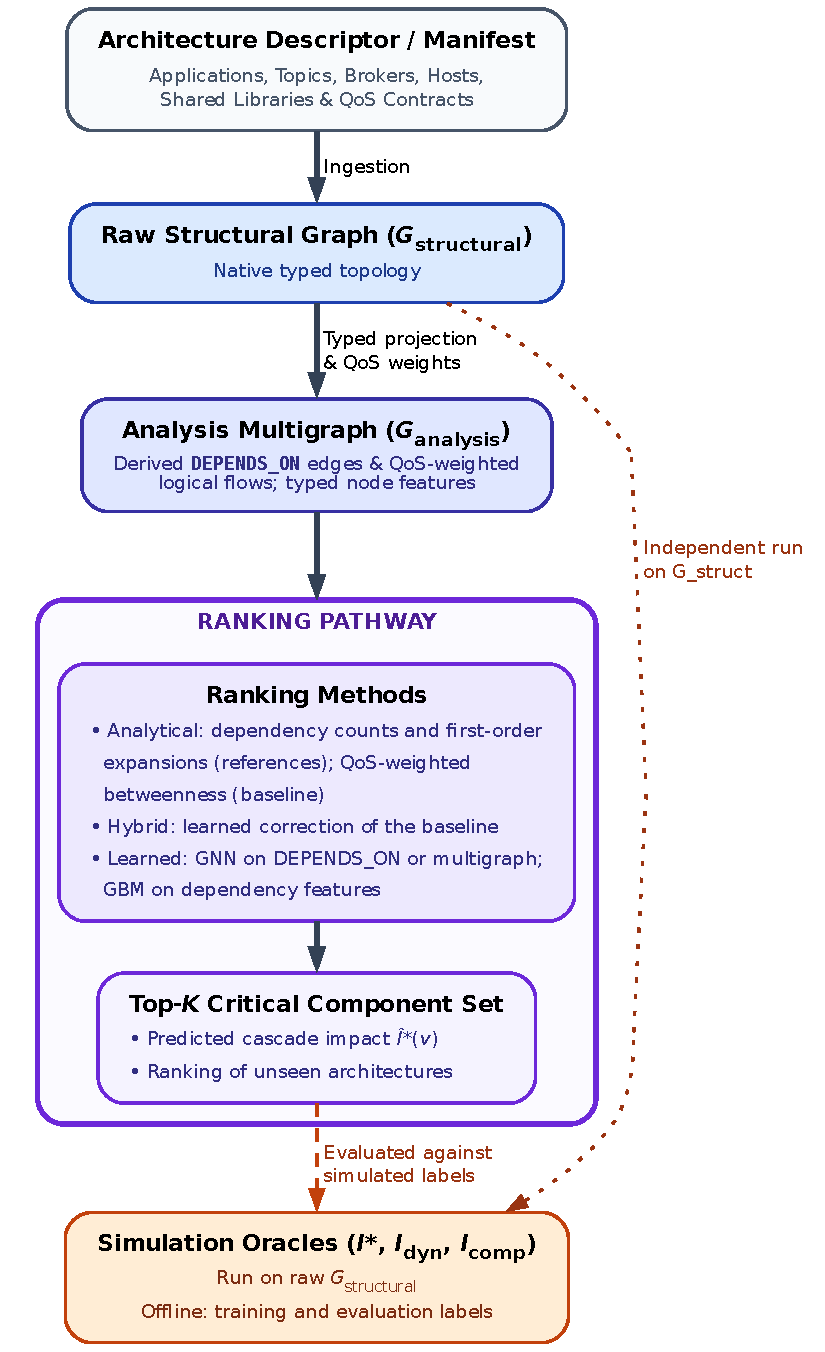
\includegraphics[width=0.70\linewidth]{figures/Figure_1}
\caption{End-to-end architecture of the SaG framework. The predictive pathway runs down the center: manifest ingestion, typed multigraph, \texttt{DEPENDS\_ON} projection with typed node properties, the ranking engines (training-free baseline, learned and hybrid; Figure~\ref{fig:engines}), and the ranked critical set. The dashed edge marks the ground-truth simulation oracles, which operate only on Gstructural, train the predictor offline, and do not participate in inference. The proposed explanation layer (not evaluated) reads the same analysis multigraph, shares no parameters with the predictor, and applies to components after they have been ranked; no predictor output flows into it.}
\label{fig:1}
\end{figure}

\subsection{Multigraph Definition}
\label{sec:3.1}

A distributed system is described as a typed, weighted, directed multigraph:

\begin{equation}
\label{eq:sag_multigraph}
\mathcal{G} = (V, E, \tau_V, \tau_E, w_V, w_E)
\end{equation}

where:

\begin{itemize}\tightlist
    \item $V = V_{\text{app}} \cup V_{\text{broker}} \cup V_{\text{topic}} \cup V_{\text{host}} \cup V_{\text{lib}}$ holds the five entity types $\mathcal{T}_V$ of Table~\ref{tab:1}; $V_{\text{host}}$ denotes physical or virtual \emph{Execution Hosts}.
    \item $E$ is the set of directed edges, and $\tau_V: V \to \mathcal{T}_V$ and $\tau_E: E \to \mathcal{T}_E$ assign entity and relation types.
    \item $w_V: V \to (0, 1]$ and $w_E: E \to (0, 1]$ weight entity criticality along with connection strength. For Applications and Libraries, $w_V(v) = 1 - \text{CQP}(v)$, where CQP is a code-quality penalty computed from static code metrics (lines of code, cyclomatic complexity, coupling and cohesion); otherwise $w_V(v) = 1.0$.
\end{itemize}

\noindent The raw multigraph is denoted $G_{\text{structural}}$ (used exclusively by simulation oracles), while $G_{\text{analysis}}$ denotes the logical \texttt{DEPENDS\_ON} projection consumed by predictors. A comprehensive reference of mathematical notation is provided in the replication repository.

\noindent\textbf{Scope of Evaluation and Entity Roles.} While the multigraph formalizes five entity types, this study concentrates its empirical study specifically on \emph{Applications} ($V_{\text{app}}$). Applications represent the developer-authored, code-level services that are often changed, refactored, and tested in CI/CD pipelines, so they are the main focus for pre-deployment triage. Brokers, Topics, Execution Hosts, and Libraries are also modeled and included because they are important for understanding indirect failure propagation. For example, we cannot analyze message routing, shared fault-domain colocation, or library-related failures without them. However, ranking infrastructure components like Brokers and Hosts is more relevant to operational provisioning than to software triage at commit time, so we treat this as a separate operational issue.

\begin{table}[htbp]
\centering
\small
\caption{Entity types and structural edge types in the SaG model.}
\label{tab:1}
\resizebox{\linewidth}{!}{%
\begin{tabular}{lll}
\toprule
\textbf{Entity Type ($\mathcal{T}_V$)} & \textbf{Architectural Role} & \textbf{Concrete System Examples} \\
\midrule
\textbf{Application} ($V_{\text{app}}$) & Process producing/consuming messages & ROS~2 node, Kafka microservice, MQTT client \\
\textbf{Broker} ($V_{\text{broker}}$) & Message routing and queuing intermediary & RabbitMQ exchange, Mosquitto, EMQX broker \\
\textbf{Topic} ($V_{\text{topic}}$) & Named logical communication channel & \texttt{/sensor/lidar}, \texttt{orders.payment.completed} \\
\textbf{Execution Host} ($V_{\text{host}}$) & Physical or virtualized execution environment & Bare-metal server, Kubernetes worker, Cloud VM \\
\textbf{Library} ($V_{\text{lib}}$) & Shared software package or runtime dependency & Kafka client, OpenCV, Protobuf runtime \\
\midrule
\textbf{Structural Edge ($\mathcal{T}_E$)} & \textbf{Direction} & \textbf{Semantic Meaning} \\
\midrule
\texttt{PUBLISHES\_TO} / \texttt{SUBSCRIBES\_TO} & App/Library $\to$ Topic & Component publishes to / consumes from topic \\
\texttt{ROUTES} & Broker $\to$ Topic & Broker manages and routes topic traffic \\
\texttt{RUNS\_ON} & App/Broker $\to$ Host & Process is hosted on host \\
\texttt{CONNECTS\_TO} & Host $\to$ Host & Network link between hosts \\
\texttt{USES} & App $\to$ Library & Application links to shared library \\
\bottomrule
\end{tabular}%
}
\end{table}

\subsection{Quality-of-Service Link Weighting}
\label{sec:3.2}

A link’s strength is determined by its Quality-of-Service (QoS) contract. For example, a \texttt{RELIABLE} topic with \texttt{TRANSIENT\_LOCAL} durability creates a stronger connection between services than a \texttt{BEST\_EFFORT} telemetry stream. Each topic $t$ has an overall weight $w(t) \in (0, 1]$ that combines its QoS policies (reliability, durability, priority) with payload size and publication frequency. We set the reliability, durability, and priority weights employing an Analytic Hierarchy Process (AHP) pairwise-comparison matrix, which we defined independently and did not adjust to fit a target vector ($CR = 0.016$, non-degenerate; the framework’s other AHP matrices also use a declared vector).

We test the effect of these weights directly on a learned ranker. When both cases include the weighted in-degree, the QoS inputs do not improve the graph neural networks on the reachability oracle (Section~\ref{sec:rq2}). However, for the queue-flow oracle, they do benefit the learned surrogate (Section~\ref{sec:rq1}). Details on how weighting affects the training-free baseline are available in the replication repository. The dependency counts reported in this paper are unweighted and do not use $w(t)$.

\subsection{Logical Dependency Projection (\texttt{DEPENDS\_ON})}
\label{sec:3.3}

Structural edges do not directly show how failures spread. For example, a subscriber depends on a publisher, but pub-sub topologies have no direct edge between them. SaG creates an explicit semantic relation called \texttt{DEPENDS\_ON}, which goes from the dependent to the dependency. This means if the target fails, the source is affected. Table~\ref{tab:2} lists the rules.

\begin{table}[htbp]
\centering
\small
\caption{The \texttt{DEPENDS\_ON} logical dependency projection rules. $^\dagger$Defined for completeness; not exercised by the Application-level evaluation.}
\label{tab:2}
\resizebox{\linewidth}{!}{%
\begin{tabular}{clll}
\toprule
\textbf{Rule} & \textbf{Dependency Category} & \textbf{Structural Pattern ($\text{Dependent} \to \text{Dependency}$)} & \textbf{Derived Weight ($w$)} \\
\midrule
\textbf{1} & \texttt{app\_to\_app} & Subscriber $\to$ Publisher (via shared Topic) & $1 - \prod_{t \in T}(1 - w(t))$ \\
\textbf{2}$^\dagger$ & \texttt{app\_to\_broker} & Publisher/Subscriber $\to$ Broker routing its topics & $1 - \prod_{t \in T}(1 - w(t))$ \\
\textbf{3}$^\dagger$ & \texttt{host\_to\_host} & Host $\to$ Host (lifted from inter-host app dependencies) & $\max_{u \in \text{hosted}(h_1), v \in \text{hosted}(h_2)} w_E(u \to v)$ \\
\textbf{4}$^\dagger$ & \texttt{host\_to\_broker} & Host $\to$ Broker (lifted from hosted app dependencies) & $\max_{u \in \text{hosted}(h)} w_E(u \to b)$ \\
\textbf{5} & \texttt{app\_to\_lib} & Application $\to$ Shared Library it \texttt{USES} & $H(w_V(\text{app}), w_V(\text{lib}))$ \\
\textbf{6}$^\dagger$ & \texttt{broker\_to\_broker} & Broker $\leftrightarrow$ Broker (shared fault-domain colocation, symmetric) & $w_V(\text{host})$ \\
\bottomrule
\end{tabular}%
}
\end{table}

Rules~1 and~2 combine topics $T$ that connect a pair using probabilistic union \cite{pearl1988probabilistic}, so that having multiple failure paths increases the connection strength. Rule~5 uses the harmonic mean $H(x, y) = 2xy/(x+y)$ \cite{hardy1952inequalities}. Rules~3 and~4 assign dependencies to hosts by taking the maximum value.

\noindent\textbf{Sequential cascades and simultaneous blasts.} Rule~1 describes sequential cascades, where if a publisher fails, its subscribers are affected because they do not receive messages. Rule~5 describes simultaneous blasts, where if a library crashes, all applications that depend on it fail at the same time. Libraries that publish or subscribe are also endpoints for Rule~1, and an Application can reach a library’s topics through Rule~5. For counting, \texttt{Topo-QoS} and all \texttt{-P} learners use Rule~1 only for direct subscriptions. The repository’s method for creating node properties also follows up to three \texttt{USES} links, so if an Application subscribes through a library it uses, it is considered a Rule~1 dependent. Rules~2, 3, 4, and~6 cover infrastructure and broker dependencies (see Table~\ref{tab:2}), which define physical host failure domains and broker routing bottlenecks. Since this evaluation focuses on Application-level code, these four rules are not used in the ranking benchmarks but are included for completeness.

\noindent\textbf{Remark 1 (the dependency count is a typed two-hop count).} Let $G_{\text{flow}}$ be the Application--Library projection (Rules~1 and~5) and $v$ an Application. By construction,
\begin{equation}
\label{eq:indeg}
\texttt{InDeg}(v) \;=\; \bigl|\{\,u \neq v : \exists t \in V_{\text{topic}},\; (v, t) \in \texttt{PUBLISHES\_TO} \wedge (u, t) \in \texttt{SUBSCRIBES\_TO}\,\}\bigr|.
\end{equation}
Since Rule~5 edges end at Libraries, every edge into an Application is a Rule~1 edge $u \to v$, which exists exactly when $u \neq v$ (an Application or a Library) directly subscribes to a topic that $v$ publishes; parallel topics collapse into one edge.

\noindent The right side of Eq.~\eqref{eq:indeg} represents publish--subscribe afferent coupling (fan-in, or the Absolute Importance of the Service \cite{martin2003agile,rud2006ais}), and is a typed two-hop query on the raw multigraph. \texttt{InDeg} can be computed directly without projection; the projection defines which typed query to use. We checked this equality on all seventeen corpus graphs, with a maximum absolute difference of $0$. We measure the extra value it adds separately: Rule~5 increases transitive reach by $+0.058$ (Section~\ref{sec:rq1}). Since the primary oracle’s first propagation wave matches this set (Section~\ref{sec:4.4}), \texttt{InDeg} and its transitive version \texttt{Reach} are used as reference points in this paper, not as predictors.

\begin{figure}[htbp]
\centering
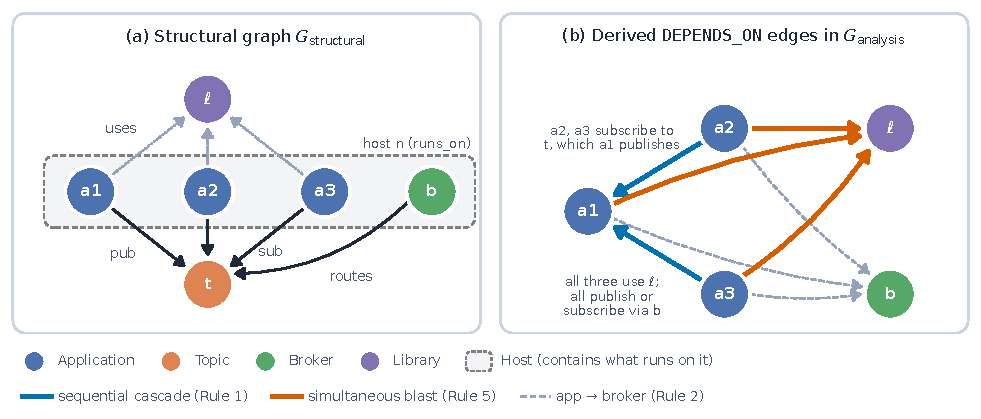
\includegraphics[width=\linewidth]{figures/Figure_2}
\caption{Running example. (a)~Three applications share topic $t$ (routed by broker $b$) and library $\ell$, and all run on host $n$. No structural edge joins two applications. (b)~The derived \texttt{DEPENDS\_ON} edges make the hidden dependencies explicit: subscribers $a_2, a_3$ depend on publisher $a_1$ (Rule~1), all applications depend on $\ell$ (Rule~5), and each application depends on the broker (Rule~2). Simulation oracles run on view~(a); predictors read view~(b).}
\label{fig:2}
\end{figure}

\subsection{Dual Graph Views}
\label{sec:3.4}

The \textbf{structural graph} $G_{\text{structural}}$ is the raw deployment topology. The \textbf{analysis graph} $G_{\text{analysis}}$ adds the \texttt{DEPENDS\_ON} edges and code metrics (see Figure~\ref{fig:2}). Predictor features are computed on $G_{\text{analysis}}$, while simulation oracles run strictly on $G_{\text{structural}}$ (Section~\ref{sec:4.4}). The two views also differ for a learner: on $G_{\text{structural}}$, every relation points away from Applications, so forward message passing does not reach them. In the \texttt{DEPENDS\_ON} graph, each Application receives messages from its dependents (Section~\ref{sec:rq2}).

\subsection{Typed Node Feature Encoding}
\label{sec:3.5}

Both the predictive pathway (Section~\ref{sec:4}) and the proposed explanation layer use typed node properties from $G_{\text{analysis}}$. All five entity types share a base set of 18 normalized topological metrics (ranging from $[0, 1]$): PageRank, Reverse PageRank, betweenness, closeness, eigenvector centrality, in-degree, out-degree, clustering, articulation, bridge ratio, node QoS weight, incoming and outgoing dependency weights, multi-path coupling, path complexity, fan-out criticality, and the Connectivity Degradation Index (CDI). We calculate four centrality features (PageRank, Reverse PageRank, betweenness, and closeness) over weighted edges, so they include QoS information. This means the so-called QoS-off condition is not entirely free of QoS effects. The in-degree feature and the incoming dependency weight $w_{\text{in}}$ (a QoS-weighted version) ensure that all learners receive information closely related to \texttt{InDeg}, so the learners inherit some overlap with the oracle’s reference counts (Section~\ref{sec:rq2}). We did not use any learner missing both columns. Type-specific blocks add more features, extending the vector to 19--25 dimensions (the full schema is in the replication repository). CDI measures structural connectivity loss using a fixed-scale breadth-first sample to keep computation time reasonable (Section~\ref{sec:rq4}). We discuss its sensitivity to hash-seeded tie-breaking in Section~\ref{sec:8.3}.

\section{Ranking Engines and Ground Truth}
\label{sec:4}

SaG uses learned engines to rank components and compares them to a training-free baseline. The learned engines are graph neural networks built on the typed multigraph and the dependency graph, as well as gradient-boosted models using per-Application dependency-graph features (Section~\ref{sec:6.2}). Hybrid engines are graph neural networks that adjust the baseline score (Section~\ref{sec:rq1-hybrid}). The training-free baseline, called \texttt{Topo-QoS}, uses QoS-weighted betweenness on the dependency projection (Section~\ref{sec:6.2}). We train or evaluate all models using simulation oracles on a separate graph view (Sections~\ref{sec:4.3}--\ref{sec:4.4}). Figure~\ref{fig:engines} illustrates the relationships between the engines and their evaluation process. Full hyperparameters and training commands are available in the experiment pages of the replication repository (Section~\ref{sec:6.1}).

\begin{figure}[htbp]
\centering
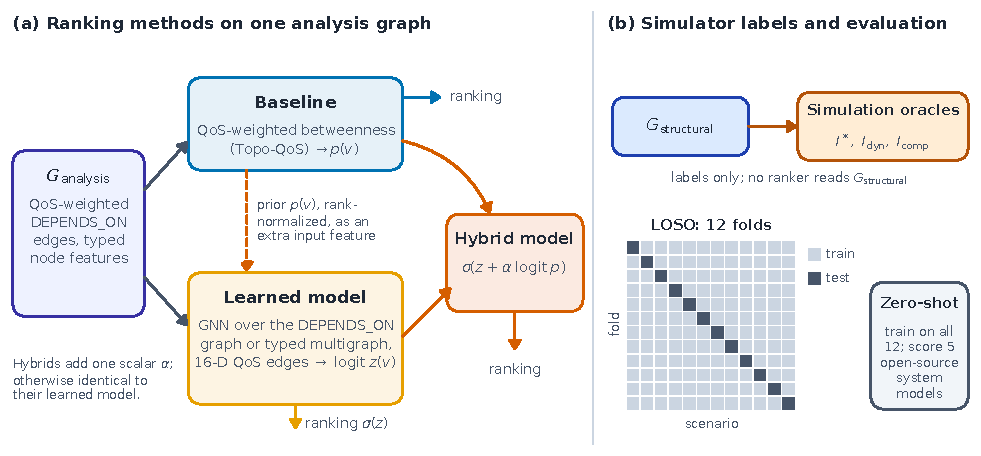
\includegraphics[width=\linewidth]{figures/Figure_3}
\caption{(a)~SaG's ranking engines read the analysis graph. The training-free baseline scores QoS-weighted betweenness; $p(v)$ is that \texttt{Topo-QoS} score, rank-normalized to $[0, 1]$ within the graph; the learned engine outputs a logit $z(v)$. A hybrid engine gives the learned engine $p(v)$ as an extra input feature and adds a learned correction to it on the logit scale, $\sigma(z + \alpha\,\operatorname{logit} p)$, with one learnable scalar $\alpha$. (b)~Ground truth comes from simulation oracles on the structural graph, which no predictor reads. We evaluate engines by leave-one-scenario-out cross-validation over twelve synthetic architectures and zero-shot on five open-source system models.}
\label{fig:engines}
\end{figure}

\subsection{Heterogeneous Graph Transformer and Attention Networks}
\label{sec:4.1}

The main learned engine, \texttt{HGT-QoS}, is a three-layer Heterogeneous Graph Transformer (HGT) \cite{hu2020hgt} built with PyTorch Geometric \cite{fey2019fast}. It uses a hidden dimension of $D=64$ and $H=4$ heads. Entity-specific linear projections map raw node features $x_v \in \mathbb{R}^{19\text{--}25}$ into the hidden space, with $h_v^{(0)} = \text{LayerNorm}(\text{GELU}(W_{\tau(v)} x_v))$. For each meta-relation $\langle \tau(u), \phi(e), \tau(v)\rangle$, attention uses type-parameterized keys, queries, and values, scaled by a learned per-meta-relation prior $\mu_{\langle \tau(u), \phi(e), \tau(v)\rangle}$; full layer-wise formulations are in the replication repository. Message passing runs over both $G_{\text{analysis}}$ and its transpose. In the raw multigraph, native relations point away from Applications, so forward message passing cannot reach the scored nodes. This means forward GNNs act as per-node MLPs over precomputed centralities (Section~\ref{sec:8.2}). The baseline Graph Attention Network (\texttt{GAT-QoS} and \texttt{GAT-P-QoS} for the dependency projection) uses a three-layer architecture with four attention heads and width $D=288$ ($D=296$ in the unweighted control for parameter matching), projecting all node types into a joint embedding space before applying homogeneous \texttt{GATConv} layers.

Each directed edge has a 16-dimensional vector. Index 0 represents the coupling weight, index 1 is the normalized path count, indices 2 to 8 are a one-hot encoding of the relation, and indices 9 to 15 are middleware QoS parameters such as reliability, durability, priority, depart-mode flag, deadline pair, and max-blocking time. The edge vector is projected and added before attention.

\subsection{Prediction Head and Training Objective}
\label{sec:4.2}

A composite head predicts the simulated cascade impact, with auxiliary heads for reliability along with maintainability. The reliability head regresses on the oracle’s reliability column; the oracle records no maintainability, so the maintainability head’s regression term is masked and trained only through the composite head. The training objective combines regression with listwise and pairwise ranking:
\begin{equation}
\label{eq:loss_active}
\mathcal{L} = \text{MSE}(\hat{I}^*, I^*) + 0.5 \cdot \text{MSE}(\hat{a}_1, I^*_R) + 0.3 \cdot \mathcal{L}_{\text{rank}} + 0.1 \cdot \mathcal{L}_{\text{pairwise}},
\end{equation}
where $\mathcal{L}_{\text{rank}}$ is ListMLE \cite{xia2008listwise} over the ground-truth permutation $\pi$,
\begin{equation}
\label{eq:listmle}
\mathcal{L}_{\text{rank}} = -\frac{1}{N}\sum_{i=1}^N \Big( \hat{s}_{\pi_i} - \log \sum_{j=i}^N \exp(\hat{s}_{\pi_j}) \Big),
\end{equation}
and $\mathcal{L}_{\text{pairwise}}$ is a margin-ranking loss with $\gamma = 0.05$ over pairs differing by more than $\gamma$. Tied labels, which affect about 31\% of Applications with $I^* = 0$, enter $\pi$ in a fixed but arbitrary order, so ListMLE is only approximately defined on them; the pairwise term ignores pairs among $\gamma$.

Models are trained with AdamW ($\eta = 3 \times 10^{-4}$, weight decay $10^{-4}$) using cosine warm restarts for up to 300 epochs. We set early stopping at 60 epochs of patience on a 20\% node-level validation split from the largest training scenario, using five fixed seeds ($\{42, 123, 456, 789, 2024\}$). We set hyperparameters and loss coefficients before the first sweep and kept them the same across all experiments. This approach differs from the registered plan, which called for selecting every hyperparameter using nested inner-LOSO selection (two-fold inner holdout). Instead, the published results use one fixed configuration, chosen during the main experiments to keep computation manageable across seeds and folds. We explain this difference in Section~\ref{sec:6.3}. We ran the registered selection later as a sensitivity analysis on the eight-configuration stage-1 grid (varying depth and rank normalization of features and labels). This analysis also used early stopping on a held-out training scenario, which is another difference from the published protocol (Section~\ref{sec:rq2}). The results confirm that the main null finding does not change under nested tuning.

\subsection{Ground-Truth Simulation Oracles}
\label{sec:4.3}

Ground truth is evaluated using simulation oracles on the raw structural multigraph $G_{\text{structural}}$:
\begin{itemize}\tightlist
    \item \textbf{Primary reachability cascade oracle ($I^*$):} Crashes component $v$, propagates outages through dependent topics, brokers and links via breadth-first traversal on $G_{\text{structural}}$, and computes the mean fractional feed loss across intact subscribers. Feed loss is scaled by a QoS severity ladder ($\times 1.2$ \texttt{RELIABLE}, $\times 1.15$ high priority, $\times 1.05$ medium) and clamped to $[0, 1]$. Each propagation wave is processed in a seeded random order, which decides ties at the propagation threshold; the label is the mean over five seeds. Disabling QoS scaling leaves the Application ordering largely intact ($\rho = 0.965$ across the twelve folds), and substituting durability-aware rescaling moves it less still ($\rho = 0.977$), showing that $I^*$ is predominantly a topological reachability metric.
    \item \textbf{Independent queue-flow discrete-event oracle ($I_{\text{dyn}}$):} A discrete-event SimPy \cite{team2020simpy} simulation to model dynamic message emission rates, queue buffer saturation, and network latency. It measures the drop in delivered message rate for surviving consumers under load, using declared rates, payload sizes, and QoS contracts that $I^*$ ignores. Its mechanism differs from reachability, but it shares the same pub-sub topology, and its first-order effect—consumers that lose a failed publisher’s messages—is again subscriber loss. While $I_{\text{dyn}}$ models declared rates and buffer limits, it operates on configured parameters free of physical operating-system dynamics like socket buffer backpressure, thread scheduling, or garbage collection pauses. It provides labels for all $1{,}321$ Applications, averaging over five seeds, and takes $12.7$ CPU-hours for the full corpus, compared to seconds for $I^*$.An earlier version used only the first $30$ Applications per fold in lexicographic order as a sensitivity check. $I_{\text{dyn}}$ agrees with $I^*$ at a mean $\rho = 0.711$ $[0.625, 0.794]$, and its published test–retest reliability is $0.74$–$0.97$, which sets the upper bound for correlation any deterministic ranker can achieve.
    \item \textbf{Composite multi-criteria failure oracle ($I_{\text{comp}}$):} An auxiliary benchmark uses the Validate-stage failure simulator. We run it on all $1{,}321$ Applications with QoS weighting and a primed baseline flow. Each removal is scored as a linear combination of four degradation components: $I_{\text{comp}}(v) = 0.35\,\text{RL}(v) + 0.25\,\text{FR}(v) + 0.25\,\text{TL}(v) + 0.15\,\text{FD}(v)$, representing Reachability Loss ($\text{RL}$), Fragmentation ($\text{FR}$; $0.70$ structural component loss $+\,0.30$ severity), TL is Throughput Loss, and FD is Flow Disruption. The weights are from one of three AHP matrices that encode a declared vector rather than elicited judgment, so $I_{\text{comp}}$ serves as a declared multi-objective stress test to assess resilience to network fragmentation and throughput disruption, rather than just subscriber loss. Since fragmentation and flow disruption occur with almost every removal, $I_{\text{comp}}(v) > 0$ for nearly every Application. $I_{\text{comp}}$ is never used as a training label.
\end{itemize}

\subsection{Input--Label Independence and Construction Bounds}
\label{sec:4.4}

Features are extracted strictly from $G_{\text{analysis}}$, while simulation oracles execute on $G_{\text{structural}}$, and no simulation output is used as an input feature; a regression test in the replication package ensures this separation.

Procedural separation does not eliminate construct overlap, which is the main risk discussed in this paper. \textbf{Criterion.} A ranking is a \emph{reference} for an oracle $O$ if it is a closed-form simplification of $O$’s own computation using the same inputs. In this case, it measures how much of $O$ comes from its own rule, not predictive skill, so comparisons are not claims of superiority. For $I^*$, the first propagation wave corresponds to the set of \texttt{InDeg} counts (see Remark~1), so the references are its first-order expansion (Eq.~\eqref{eq:analytic_istar}), \texttt{InDeg}, \texttt{Reach}, and their raw-graph equivalents. For $I_{\text{dyn}}$, no ranking truncates its computation, but its main effect is still subscriber loss, so we use the same rankings as references here too. For $I_{\text{comp}}$ no ranking is a truncation either; its fragmentation and flow terms respond to removing high-degree and high-betweenness nodes, so \texttt{Topo-QoS} and raw degree are considered close to it, and their performance is interpreted with the same caution as the references for $I^*$. The learned engines are not references by this definition, but they use in-degree features and are trained on $I^*$, so they share some overlap (Section~\ref{sec:rq2} measures this). Two analyses limit the circularity instead of removing it. Every ranker is evaluated on all three oracles, and its agreement with $I_{\text{dyn}}$ is also reported after removing the effect of $I^*$ (and separately, the first-order term) (Section~\ref{sec:rq1}). However, none of these analyses replaces validation against real failures in live distributed systems, which this study does not include (Section~\ref{sec:8.3}). Therefore, all results depend on the simulations' accuracy.

\section{Experimental Setup}
\label{sec:6}

\subsection{Corpus and Replication Package}
\label{sec:6.1}

The corpus includes 2,812 components from seventeen architectures (see Table~\ref{tab:4}). Twelve synthetic topologies make up the LOSO folds, covering areas like autonomous vehicles, financial trading, healthcare, industrial SCADA, smart-city IoT, telecom RAN, logistics, gaming, microservices, enterprise integration, and air-traffic management. Because all twelve topologies and their code metrics come from the same family, LOSO tests transfer across several parameter settings of that generator, not across unrelated industrial systems. We can regenerate each topology exactly from its configuration, and continuous integration checks this using a SHA-256 manifest.

\begin{table}[htbp]
\centering
\small
\caption{Evaluation corpus. The twelve synthetic topologies are the LOSO folds; we exclude the five open-source system models from all training and use them only for zero-shot transfer (Section~\ref{sec:rq3}). Counts are read from the committed topology files and verified in CI; the replication repository details per-scenario composition.}
\label{tab:4}
\begin{tabular}{lrrrrrrr}
\toprule
\textbf{Dataset} & \textbf{$|V|$} & \textbf{$|V_{\text{app}}|$} & \textbf{Topics} & \textbf{Brokers} & \textbf{Hosts} & \textbf{Libs} & \textbf{$|E|$} \\
\midrule
Synthetic evaluation scenarios (11) & 2{,}387 & 1{,}295 & 588 & 60 & 194 & 250 & 10{,}657 \\
Synthetic case study — ATM (1)    &    74 &    26 &  27 &  5 &   8 &   8 &   261 \\
\midrule
\textbf{Synthetic subtotal (12 LOSO folds)} & \textbf{2{,}461} & \textbf{1{,}321} & \textbf{615} & \textbf{65} & \textbf{202} & \textbf{258} & \textbf{10{,}918} \\
\textbf{Open-source system models (5)}    & \textbf{351}    &   \textbf{141} & \textbf{120} & \textbf{16} &  \textbf{32} &  \textbf{42} & \textbf{700} \\
\midrule
\textbf{Total} & \textbf{2{,}812} & \textbf{1{,}462} & \textbf{735} & \textbf{81} & \textbf{234} & \textbf{300} & \textbf{11{,}618} \\
\bottomrule
\end{tabular}
\end{table}

The five open-source systems are hand-crafted models. Autoware.universe (ROS~2), EdgeX Foundry, Home Assistant, and two meshes based on Online Boutique and Train-Ticket were each created by a single author as typed multigraphs using public architectural documentation. We did not mechanically extract them from source code or container manifests. Because one person modeled them, bias is possible, and we cannot measure inter-rater agreement. Some details, like brokers, QoS profiles, code metrics, and host specifications, are partly assumed. Two models differ significantly from their originals: the Online Boutique model is a 22-application pub-sub mesh with four brokers, while the original utilizes RPC and has no broker. The Train-Ticket model treats its service-discovery registry as an event broker. In both cases, we changed synchronous RPC interactions to asynchronous request-and-response topics with routing intermediaries (see Supplementary Section~S.36). This preserves the direction of dataflow but changes synchronous blocking calls into decoupled event streams, leaving out client-side timeout and thread-pool exhaustion effects. Neither model includes synchronous call edges. As a result, RQ3 tests zero-shot transfer to stylized architecture models inspired by open-source systems made by a single modeler, not to real production systems or automatically extracted call graphs.

Replication package. All datasets, harnesses, checkpoints, and result artifacts are stored on Zenodo (see Data Availability). In addition, the public repository provides documentation for each experiment, including its protocol, hyperparameters, \texttt{make} target, artifacts, and extended results (\sagexperiments).

\subsection{Predictors}
\label{sec:6.2}

Table~\ref{tab:predictor_taxonomy} shows the predictors: the training-free baseline (Topo-QoS), learned models on the dependency graph and raw multigraph, and hybrid models. Other training-free baselines (Degree-raw, PR-raw, RevPR-raw, Topo) are available in the replication repository. Dependency counts are not included in the table because they repeat the main oracle’s propagation rule and are reported as reference rankings below. For GNNs, '-QoS' means using the 16-dimensional QoS edge vector (see Section~\ref{sec:4.1}) along with three QoS node columns ($w$, $w_{\text{in}}$, $w_{\text{out}}$). 'Hybrid-X' refers to engine X adjusted by the baseline prior. GAT and GAT-QoS are untyped GATs with the same parameter budget as HGT, and GAT-QoS uses the same 16-D edge vector as HGT-QoS. Together, these define a 2x2 grid based on typing (GAT vs.\ HGT) and the QoS channel. The study also tested smaller and projection-based variants, which are listed in the replication repository. The learned and hybrid models use the native typed multigraph under LOSO, while the '-P' models use the Application–Library \texttt{DEPENDS\_ON} graph, with identical graph node features and labels. In QoS-off settings, all edge weights are set to 1, and the QoS node columns are set to zero, but four centralities still use QoS (see Section~\ref{sec:3.5}).

\begin{table}[htbp]
\centering
\small
\caption{Predictors reported in the main text. \texttt{-QoS}: QoS-weighted distances (\texttt{Topo-QoS}) or the 16-D QoS edge vector plus three QoS node columns (GNNs); \texttt{-P}: trained on the derived dependency graph; \texttt{Hybrid-X}: engine X corrected by the \texttt{Topo-QoS} prior (the supplementary variant \texttt{GAT-P+InDeg} incorporates the \texttt{InDeg} reference prior). Unsuffixed GNNs (\texttt{GAT}, \texttt{HGT}) serve as raw-multigraph confound controls ($G_{\text{structural}}$). $^\P$\texttt{Topo-QoS} carries an implementation defect where the articulation point term is zero (corrected score is $0.533$). Reference rankings that restate the oracle (Analytic $I^*$, \texttt{InDeg}, \texttt{Reach}) and \texttt{GAT-P+InDeg}, which uses one as its prior, are not predictors. We archive other training-free baselines and exploratory raw-graph references (Pubs-raw, Reach-R1) in the replication repository. Each dependency-graph learner keeps the architecture and parameter budget of its raw-multigraph counterpart.}
\label{tab:predictor_taxonomy}
\resizebox{\linewidth}{!}{%
\begin{tabular}{lllr}
\toprule
\textbf{Predictor} & \textbf{Graph read} & \textbf{Typing / edge input} & \textbf{Params} \\
\midrule
\multicolumn{4}{l}{\textit{Training-free baseline (registered comparator)}} \\
\texttt{Topo-QoS}$^\P$ & App--Lib \texttt{DEPENDS\_ON} & scalar $w(e)$; betweenness only (AP term zero; corr.\ $0.533$) & 0 \\
\midrule
\multicolumn{4}{l}{\textit{Learned, dependency graph}} \\
\texttt{GAT-P-QoS}, \texttt{HGT-P-QoS} & App--Lib \texttt{DEPENDS\_ON} & homogeneous / heterogeneous & 429{,}992 / 434{,}620 \\
\midrule
\multicolumn{4}{l}{\textit{Learned, raw multigraph: typing $\times$ QoS channel at matched budget}} \\
\texttt{GAT} / \texttt{GAT-QoS} & $G_{\text{structural}}$ + features & homogeneous; none / 16-D & 437{,}496 / 429{,}992 \\
\texttt{HGT} / \texttt{HGT-QoS} & $G_{\text{structural}}$ + features & heterogeneous; 1-hot / 16-D & 434{,}620 \\
\texttt{Hybrid-GAT} / \texttt{Hybrid-HGT} & $G_{\text{structural}}$ + features & as base + \texttt{Topo-QoS} prior & 431{,}433 / 434{,}941 \\
\bottomrule
\end{tabular}%
}
\end{table}

\noindent\textbf{Training-free baseline.} \texttt{Topo-QoS} is computed on the Application--Library \texttt{DEPENDS\_ON} graph (Rules 1 and 5):
\begin{equation}
\label{eq:topo}
\text{Topo-QoS}(v) = 0.6 \cdot \text{BT}_{w}(v) + 0.4 \cdot \text{AP}(v),
\end{equation}
where $\text{BT}_{w}$ is betweenness over edge distances $d(e) = 1/(w(e) + 10^{-6})$, so tightly coupled edges attract shortest paths, and AP flags articulation points. Because of an implementation defect, the articulation term reads zero for every node, so the reported score ranks as QoS-weighted betweenness. Restoring the term lowers \texttt{Topo-QoS} from $0.553$ to $0.533$, so the defect does not favor the reference counts. We archive the unweighted Topo baseline in the replication repository.

Three primary training-free rankings restate the reachability oracle’s propagation rule and are reported as references: the first-order expansion of $I^*$ (Analytic $I^*$, Eq.~\eqref{eq:analytic_istar}); \texttt{InDeg}$(v)$, the number of direct dependents of $v$ on the Application--Library \texttt{DEPENDS\_ON} graph, which for an Application equals publish–subscribe afferent coupling and is exactly the set $I^*$'s first wave reaches (Remark~1); and \texttt{Reach}$(v)$, the number of its transitive dependents normalized by $|V| - 1$, which is the set a reachability cascade can visit. In addition, we archive raw-multigraph topic counts (Pubs-raw) and transitive closure without Rule~5 (Reach-R1) in the replication repository. A reference shows how much of an oracle a restatement of its rule recovers, which is the size of the circularity, not predictive skill. References carry no contrast against \texttt{Topo-QoS}, and a learner’s distance from them is reported as such, not as a test.

\subsection{Metrics, Protocols and Statistics}
\label{sec:6.3}

\noindent\textbf{Population.} Every predictor is scored on the Application set $V_{\text{app}}$.

Metrics. We use Spearman $\rho$ to measure ranking against the simulation oracles. To distinguish between active components and those with zero impact, we report both the full-population Spearman $\rho$ and the active-stratum Spearman $\rho_{>0}$, which only includes components with true impact greater than zero. To identify critical sets, we use Overlap@$K$, the fraction of the true top-$K$ recovered by the predicted top-$K$, where $K$ is about 20\% of $|V_{\text{app}}|$. We also report PR-AUC, $F_1@\tau$, and nDCG@10 in the replication repository.

Protocols. In the LOSO setup, we train learned models on eleven scenarios and test on the twelfth, repeating this for all 12 folds and five random seeds. The reported value is the average $\rho$ across seeds. For zero-shot transfer, we evaluate models built on all twelve scenarios across the five system models without any fine-tuning. Training-free rankers are not fitted to any data, so for them, both protocols become per-scenario analyses on the same twelve scenarios and five models. We include them in the same tables to ensure every row is scored on the same scenarios and labels.

Statistics. The summary $\rho$ is the average Spearman correlation for each fold or system, with a 95\% confidence interval from a bootstrap that resamples folds ($B = 2{,}000$) \cite{efron1993introduction}. We compare results using paired two-sided Wilcoxon signed-rank tests across folds \cite{wilcoxon1945individual}. With 12 folds, the smallest possible two-sided $p$-value is $0.00049$. Fisher-$z$ averaging does not change the row order in Table~\ref{tab:hybrid}. Weighting folds by $|V_{\text{app}}|$ keeps the top five the same (the reference \texttt{InDeg} rises to $0.810$) but increases \texttt{Topo-QoS} to $0.596$, corresponding to the raw-multigraph learned engines ($0.595$--$0.606$). Spearman $\rho$ gives tied scores their average rank. Overlap@$K$ breaks ties at the $K$ boundary by node order, which is arbitrary for integer counts, so Section~\ref{sec:rq1} also reports tie-aware recall curves. Because LOSO folds share ten of eleven training scenarios, we also test every registered contrast with the Nadeau--Bengio corrected resampled $t$-test \cite{nadeau2003inference} and, when weighting by $|V_{\text{app}}|$, with an exact sign-flip permutation test.

\noindent\textbf{Analysis plan and the status of each result.} The evaluation protocol is version-controlled in the replication repository. We registered fourteen numbered amendments across the study, encompassing sensitivity, ablation, and reclassification arms, with none withheld. We assign every reported result to one of three tiers. \emph{Confirmatory}: the original plan's primary contrast (\texttt{HGT-QoS} vs.\ \texttt{Topo-QoS}) and unweighted contrast (\texttt{HGT} vs.\ \texttt{Topo-QoS}), Holm-corrected across the two. \emph{Registered secondary}: hypotheses committed before their respective arms executed---including the matched $2\times2$, hybrid engines, reference counts, dependency-graph learners, derivation value, full-population queue-flow labels, and sensitivity arms, each Holm-corrected within its family. We conducted all secondary analyses after observing the primary null. \emph{Exploratory}: post hoc investigations and reference reclassifications (which altered no figures; Section~\ref{sec:4.4}). \textbf{Plan deviation}: the registered nested inner selection was simplified to a fixed configuration during primary sweeps; a sensitivity analysis assesses the registered selection (Section~\ref{sec:rq2}). Because sequential amendment registration accumulates family-wise error throughout rounds, we also evaluate an omnibus Holm correction across all 13 decision-bearing contrasts (Supplementary Table~\ref{tab:supp-omnibus}; \path{reproduce/omnibus_holm.py}). Both hybrid contrasts against \texttt{Topo-QoS} remain significant under this omnibus adjustment (Hybrid-GAT $p_{\text{omni}} = 0.019$, Hybrid-HGT $p_{\text{omni}} = 0.041$). In contrast, the primary contrast remains null ($+0.069$, nominal $p = 0.266$, $p_{\text{omni}} \ge 0.46$). Main-text tables report per-family Holm corrections to reflect the pre-specified hypothesis families.

\section{Results}
\label{sec:7}

All results are reported on the Application population ($V_{\text{app}}$) against the primary oracle $I^*(v)$, and, for the rankers of Table~\ref{tab:independent_oracles}, also against the queue-flow oracle $I_{\text{dyn}}(v)$ and the multi-criteria oracle $I_{\text{comp}}(v)$ (Section~\ref{sec:4.3}). Only the primary and secondary contrasts are confirmatory; every other contrast is registered as secondary or exploratory (Section~\ref{sec:6.3}). Per-fold results, secondary strata, and extended protocol notes are in the public experiment pages (Section~\ref{sec:6.1}). Figure~\ref{fig:results} summarizes the main findings.

\begin{figure}[htbp]
\centering
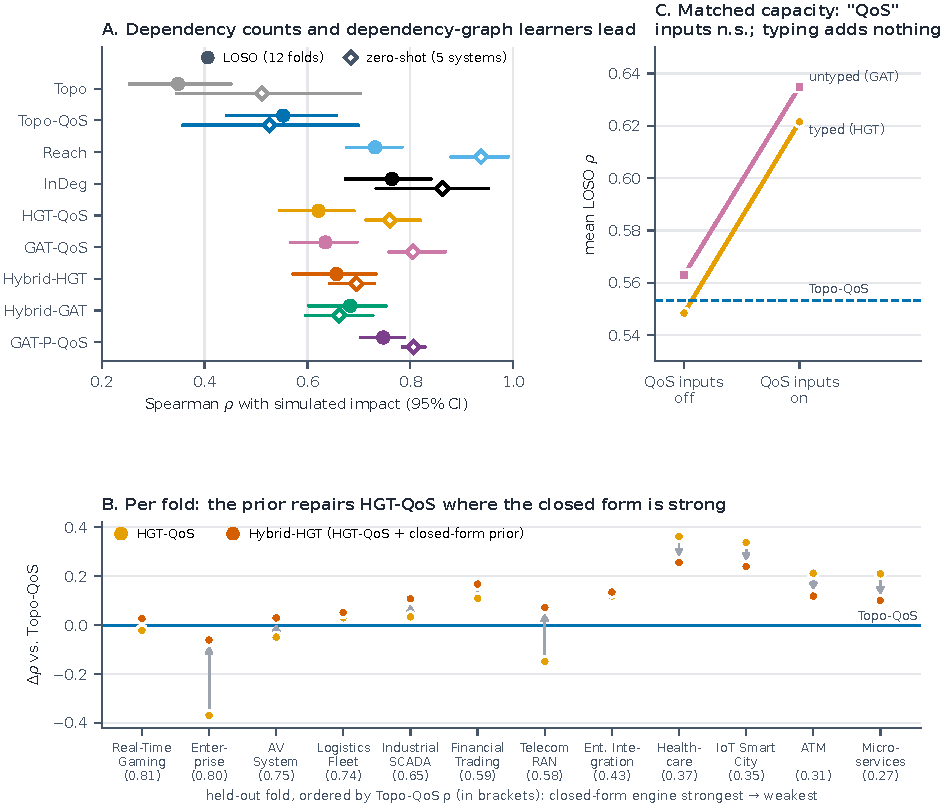
\includegraphics[width=\linewidth]{figures/Figure_5}
\caption{Main results for the Application population. (A)~Shows the mean Spearman $\rho$ with 95\% bootstrap intervals under LOSO (filled circles; see Table~\ref{tab:hybrid}) and zero-shot results on five system models (open diamonds). Grey hollow markers represent reference rankings that restate $I^*$'s propagation rule (\texttt{InDeg}, \texttt{Reach}) and are not predictors. The neural model using the dependency graph (\texttt{GAT-P-QoS}) performs similarly to \texttt{InDeg}; the two are statistically similar but not identical. (B)~Shows the improvement of \texttt{HGT-QoS} and Hybrid-HGT over \texttt{Topo-QoS} for each held-out fold. (C)~Displays cell means from the capacity- and channel-matched 2 $\times$ 2 (Table~\ref{tab:contrasts_matched}): the ``QoS'' inputs, which include a QoS-weighted in-degree column, increase both models by about 0.07 (not significant after Holm correction), while typed and untyped configurations show no difference. When $w_{\text{in}}$ is held in both arms, the ``QoS'' effect drops to +0.030 (Table~\ref{tab:a14}).}
\label{fig:results}
\end{figure}

\subsection{RQ1: Ranking Accuracy of Learned Engines}
\label{sec:rq1}
\label{sec:rq1-hybrid}
\label{sec:rq1-loso}

\paragraph{Summary} \emph{Using derived dependency graphs allows for highly accurate cascade-impact ranking. The graph attention network (\texttt{GAT-P-QoS}) achieves $\rho = 0.748$ against the primary reachability oracle $I^*$. Causal ablation tests show this strong performance comes from representing the degree distribution (losing $0.14$ without degree features; see Section~\ref{sec:rq2}), corresponding to the first-order reference level ($0.764$, statistically similar but not equivalent within $\pm 0.05$). For the more expensive queue-flow oracle $I_{\text{dyn}}$ ($12.7$ CPU-hours), a learned surrogate using dependency-graph features reaches $\rho = 0.799$, considerably outperforming all closed-form approximations ($0.706$, Holm $p = 0.019$) and capturing declared QoS signals ($+0.095$). Under multi-criteria failure conditions ($I_{\text{comp}}$), hybrid engines remain stable ($0.58$) while pure neural models drop sharply ($0.144$--$0.334$). On the raw multigraph, the main registered comparison (\texttt{HGT-QoS} vs. \texttt{Topo-QoS}, $0.553$; corrected $0.533$) showed no significant difference ($\Delta\rho = +0.069$, $p = 0.266$). To recover $80\%$ of the true top-$20\%$ set, \texttt{GAT-P-QoS} must flag the top $40\%$.}

Learned engines are trained on eleven scenarios and scored on the twelfth; training-free rankers are scored on all twelve (26 to 300 Applications, $K$ between 5 and 60). Table~\ref{tab:hybrid} reports all of them against $I^*$, with the reference rankings of Section~\ref{sec:6.2} in a separate block: they restate $I^*$'s rule, so their rows measure the circularity and carry no contrast.

\begin{table}[htbp]
\centering
\small
\caption{Main results under LOSO across twelve synthetic architectures (Application population; learned engines: five seeds, CPU sweeps). $\Delta\rho$ is paired by fold against \texttt{Topo-QoS}, with a bootstrap 95\% CI ($B = 2{,}000$) and a two-sided Wilcoxon signed-rank test. $\rho_{>0}$ denotes Spearman correlation restricted to active components ($I^* > 0$). $p_{\text{Holm}}$ is given within each registered family: hybrids (registered secondary). The reference block holds canonical rankings that restate $I^*$'s propagation rule (the post hoc first-order expansion, Eq.~\eqref{eq:analytic_istar}; the dependency counts); they are not predictors and carry no contrast. $^\ddagger$Exploratory: contrasts against the references and raw counterparts. Note: \texttt{Topo-QoS} carries an implementation defect (articulation term zero; Section~\ref{sec:6.2}); corrected value is $0.533$. Additional training-free baselines and exploratory raw-graph references (Pubs-raw, Reach-R1, Degree-raw, RevPR-raw, Topo), per-fold values, contrasts among references, and \texttt{GAT-P+InDeg} are provided in the replication repository. Underlined: best predictor per column.}
\label{tab:hybrid}
\resizebox{\linewidth}{!}{%
\begin{tabular}{lcccccc}
\toprule
\textbf{Predictor} & \textbf{LOSO $\rho$ [95\% CI]} & \textbf{Active $\rho_{>0}$} & \textbf{$\Delta\rho$ vs \texttt{Topo-QoS} [95\% CI]} & \textbf{Won} & \textbf{$p$ ($p_{\text{Holm}}$)} & \textbf{Overlap@$K$} \\
\midrule
\multicolumn{7}{l}{\textit{Reference: restatements of $I^*$'s propagation rule (not predictors)}} \\
\textbf{Analytic $I^*$} & 0.808 $[0.755, 0.853]$ & 0.631 & --- & --- & --- & 0.536 \\
\textbf{InDeg (direct dependents)} & 0.764 $[0.674, 0.840]$ & 0.516 & --- & --- & --- & 0.504 \\
\textbf{Reach (transitive dependents)} & 0.732 $[0.674, 0.782]$ & 0.286 & --- & --- & --- & 0.344 \\
\midrule
\multicolumn{7}{l}{\textit{Training-free baseline (registered comparator)}} \\
\textbf{Topo-QoS} & 0.553 $[0.443, 0.657]$ & 0.280 & --- & --- & --- & 0.388 \\
\midrule
\multicolumn{7}{l}{\textit{Learned, on the dependency graph}} \\
\textbf{GAT-P-QoS} & \underline{0.748} $[0.704, 0.789]$ & \underline{0.440} & $\underline{+0.195}$ $[+0.100, +0.294]$ & 10/12 & 0.0068$^\ddagger$ & \underline{0.454} \\
\textbf{HGT-P-QoS} & 0.514 $[0.392, 0.636]$ & 0.237 & $-0.039$ $[-0.155, +0.077]$ & 4/12 & 0.622$^\ddagger$ & 0.380 \\
\midrule
\multicolumn{7}{l}{\textit{Learned and hybrid, on the raw multigraph}} \\
\textbf{HGT-QoS} & 0.622 $[0.547, 0.690]$ & 0.312 & $+0.069$ $[-0.046, +0.174]$ & 8/12 & 0.266 & 0.426 \\
\textbf{GAT-QoS} & 0.635 $[0.567, 0.696]$ & 0.338 & $+0.082$ $[-0.046, +0.201]$ & 7/12 & 0.233 & 0.438 \\
\textbf{Hybrid-HGT} & 0.657 $[0.572, 0.733]$ & 0.345 & $+0.103$ $[+0.055, +0.152]$ & 11/12 & 0.0034 (0.0068) & 0.435 \\
\textbf{Hybrid-GAT} & 0.683 $[0.603, 0.753]$ & 0.362 & $+0.130$ $[+0.075, +0.190]$ & 11/12 & 0.0015 (0.0029) & 0.450 \\
\bottomrule
\end{tabular}%
}
\end{table}

\noindent\textbf{The reference level.} As noted in Remark~1, \texttt{InDeg} represents publish--subscribe afferent coupling \cite{martin2003agile,rud2006ais,bogner2017maintainability} and counts exactly the Applications reached by the first propagation wave of $I^*$. \texttt{Reach} counts the transitive dependents that a reachability cascade can visit. Their values on $I^*$ ($0.764$, $\rho_{>0} = 0.516$; $0.732$) show how much of the oracle is recovered by expressing again its rule, rather than measuring predictive skill. Exploratory raw-multigraph references are evaluated in the replication repository: counting published topics (Pubs-raw) achieves $0.731$, and transitive closure without Rule~5 (Reach-R1) gets $0.674$. Among the references, that derivation matters in one case: without Rule~5, \texttt{Reach} drops by $0.058$ (9/12 folds, Holm $p = 0.0068$; derivation ablation). Untyped raw-graph metrics do not recover the reference: total degree reaches $0.199$ and reverse PageRank $0.089$, while PageRank is constant for every Application because they have no incoming raw edges.

\noindent\textbf{The first-order expansion of the oracle.} The strongest reference is a post hoc closed-form first-order expansion of $I^*$:
\begin{equation}
\label{eq:analytic_istar}
\hat{I}^*_1(v) = \sum_{t \in \text{pub}(v)} \frac{|\text{sub}(t)|}{|\text{pub}(t)|},
\end{equation}
where $|\text{pub}(t)| \ge 1$ holds for all published topics $t \in \text{pub}(v)$ by construction ($v$ publishes to $t$), preventing any division by zero. It reaches mean $\rho = 0.808$ $[0.755, 0.853]$ ($\rho_{>0} = 0.631$): direct subscriber loss is most of what $I^*$ measures, and \texttt{InDeg} is a coarser version of the same quantity. As a reference, it bounds the mean rather than every fold: on four folds (AV, Financial Trading, Healthcare, Industrial SCADA), \texttt{InDeg} slightly exceeds it (by $0.005$--$0.038$).

\noindent\textbf{Learners on the dependency graph approach the reference.} The same graph neural networks, after being trained on the dependency graph instead of the raw multigraph, achieve $\rho = 0.748$ (\texttt{GAT-P-QoS}), making it the best GNN in Table~\ref{tab:hybrid}. This is $0.016$ below the direct-dependent count for individual seeds, and the five-seed ensemble is $0.007$ above it ($0.772$, Table~\ref{tab:independent_oracles}). These differences are not statistically significant, nor do they show equivalence: the $90\%$ interval of the per-fold difference is $\pm 0.076$, so a two one-sided test at the registered margin of $\pm 0.05$ does not pass ($p = 0.17$ per seed, $0.13$ for the ensemble; equivalence arm F3). At this sample size, the learner and the count are indistinguishable and not ranked. The closeness to the reference depends on the degree features each learner receives (Section~\ref{sec:3.5}): removing \texttt{in\_degree} and $w_{\text{in}}$ lowers \texttt{GAT-P-QoS} to $0.612$ (Section~\ref{sec:rq2}). We archive a version that uses \texttt{InDeg} as its prior in the replication repository, since it is a reference prior. \texttt{HGT-P-QoS} only reaches $0.514$ and is highly dependent on the seed (mean within-fold seed SD $0.254$; Section~\ref{sec:8.3}).

\noindent\textbf{Hybrid engines secure statistically significant gains beyond baseline priors.} Hybrid-HGT achieves $\rho = 0.657$ ($+0.103$, Holm $p = 0.0068$) and Hybrid-GAT reaches $0.683$ ($+0.130$, Holm $p = 0.0029$) compared to \texttt{Topo-QoS}, each outperforming the baseline in 11 out of 12 folds. Both results remain statistically significant under the omnibus Holm correction ($p_{\text{omni}} = 0.041$ and $0.019$), the Nadeau--Bengio corrected $t$ ($p = 0.019$ and $0.014$), and $|V_{\text{app}}|$-weighted averaging (exact sign-flip $p = 0.038$ and $0.005$). In this comparison, a hybrid uses $p(v)$ as an input and adds a learned correction to its logit, nesting its comparator. When compared to their own base learners, neither hybrid shows a significant difference (Hybrid-HGT vs. \texttt{HGT-QoS} $+0.035$, $p = 0.73$; Hybrid-GAT vs. \texttt{GAT-QoS} $+0.048$, $p = 0.30$). The prior also reduces transfer performance: in zero-shot tests, both hybrids perform worse than their base learners (Section~\ref{sec:rq3}). On their own, the raw-multigraph learned engines do not differ significantly from \texttt{Topo-QoS} (\texttt{HGT-QoS} $+0.069$, $p = 0.266$; \texttt{GAT-QoS} $+0.082$, $p = 0.233$).

\begin{table}[htbp]
\centering
\small
\caption{Rankers against three oracles, twelve LOSO folds, Application population (registered secondary and exploratory). All three oracles are exhaustive over the $1{,}321$ Applications; $I_{\text{dyn}}$ is the five-seed mean across all components. Partial $\rho$: Spearman correlation with $I_{\text{dyn}}$ after the rank of $I^*$, or of the first-order expansion $\hat{I}^*_1$ (Eq.~\eqref{eq:analytic_istar}), is regressed out of both. Published learned rows score the mean of the five seeds' \emph{predictions}, which raises $\rho$ on $I^*$ above the per-seed means of Table~\ref{tab:hybrid}; the GBM surrogate rows and GAT surrogate are per-seed means. $^\star$Trained on $I_{\text{dyn}}$ labels of the eleven training scenarios: a surrogate for $I_{\text{dyn}}$, not an independent check of it. Reference rows restate $I^*$'s rule (Section~\ref{sec:4.4}). (For \texttt{Topo-QoS}, the corrected $I^*$ value is $0.533$; Section~\ref{sec:6.2}.) Underlined: highest value per column among predictors. 95\% CIs are bootstrapped across folds.}
\label{tab:independent_oracles}
\resizebox{\linewidth}{!}{%
\begin{tabular}{lccccc}
\toprule
\textbf{Ranker} & $I^*$ $\rho$ & $I_{\text{dyn}}$ $\rho$ [95\% CI] & Partial $\rho(\cdot, I_{\text{dyn}} \mid I^*)$ [95\% CI] & Partial $\rho(\cdot, I_{\text{dyn}} \mid \hat{I}^*_1)$ & $I_{\text{comp}}$ $\rho$ \\
\midrule
\multicolumn{6}{l}{\textit{Reference: restatements of $I^*$'s propagation rule (not predictors)}} \\
\textbf{Analytic $I^*$} & 0.808 & 0.706 $[0.629, 0.783]$ & 0.318 $[0.234, 0.412]$ & --- & 0.636 \\
\textbf{InDeg} & 0.764 & 0.664 $[0.562, 0.758]$ & 0.272 $[0.188, 0.366]$ & 0.079 & 0.650 \\
\textbf{Reach} & 0.732 & 0.583 $[0.510, 0.651]$ & 0.117 $[0.055, 0.184]$ & 0.102 & 0.302 \\
\midrule
\multicolumn{6}{l}{\textit{Training-free baseline}} \\
\textbf{Topo-QoS} & 0.553 & 0.471 $[0.381, 0.559]$ & 0.134 $[0.061, 0.204]$ & $-0.091$ & \underline{0.702} \\
\midrule
\multicolumn{6}{l}{\textit{Learned GNNs (seed ensemble)}} \\
\textbf{GAT-P-QoS} & 0.772 & 0.615 $[0.549, 0.673]$ & 0.111 $[0.016, 0.213]$ & 0.182 & 0.274 \\
\textbf{Hybrid-GAT} & 0.702 & 0.599 $[0.514, 0.669]$ & \underline{0.173} $[0.082, 0.267]$ & 0.056 & 0.585 \\
\textbf{Hybrid-HGT} & 0.672 & 0.573 $[0.497, 0.638]$ & 0.162 $[0.074, 0.252]$ & 0.029 & 0.582 \\
\textbf{HGT-QoS} & 0.667 & 0.549 $[0.464, 0.622]$ & 0.130 $[0.035, 0.224]$ & 0.212 & 0.201 \\
\textbf{GAT-QoS} & 0.647 & 0.523 $[0.436, 0.606]$ & 0.107 $[0.018, 0.199]$ & \underline{0.217} & 0.144 \\
\textbf{HGT-P-QoS} & 0.618 & 0.496 $[0.395, 0.601]$ & 0.112 $[0.033, 0.190]$ & 0.087 & 0.334 \\
\midrule
\multicolumn{6}{l}{\textit{Dynamic queue-flow surrogates (trained on $I_{\text{dyn}}$)}} \\
\textbf{GBM-P-QoS$\to$dyn$^\star$} & \underline{0.764} & \underline{0.799} & --- & --- & 0.477 \\
\textbf{GAT-P-QoS$\to$dyn$^\star$} & 0.734 & 0.598 & --- & --- & 0.368 \\
\bottomrule
\end{tabular}%
}
\end{table}

\noindent\textbf{Beyond the reachability oracle.} Table~\ref{tab:independent_oracles} compares the rankers against two other oracles. On the full-population $I_{\text{dyn}}$, which matches $I^*$ at $\rho = 0.711$ $[0.625, 0.794]$, the reference methods outperform all GNNs (first-order expansion $0.706$, \texttt{InDeg} $0.664$, compared to $0.496$--$0.615$ for GNNs), and \texttt{Topo-QoS} achieves $0.471$. Since $I_{\text{dyn}}$ shares its topology and first-order effect with $I^*$, the partial correlation shows how much of each ranking remains after removing the oracle it was fitted to or restates. After removing the rank of $I^*$, \texttt{InDeg} keeps $0.272$ $[0.188, 0.366]$, \texttt{Reach} $0.117$, \texttt{Topo-QoS} $0.134$, and the GNNs $0.107$--$0.173$, with all intervals excluding zero. If we remove the first-order expansion instead, the order reverses: \texttt{InDeg} stays at $0.079$. Meanwhile, the raw-multigraph GNNs keep most of their value ($0.212$--$0.217$), showing that the learners capture queue-flow signals beyond what the direct count provides. Learning from the right labels is more important than the graph model itself. A gradient-boosted model using counts, the first-order expansion, and QoS features, trained on $I_{\text{dyn}}$ labels, ranks held-out architectures at $0.799$, outperforming the first-order expansion ($+0.094$, Holm $p = 0.019$) and \texttt{InDeg} ($+0.135$, Holm $p = 0.019$; Family B). Its QoS features provide this gain ($+0.095$ over the same model without them, Holm $p = 0.014$), while on $I^*$ they add nothing ($-0.003$, $p = 0.62$; Family C). The GNN trained on the same labels does not: \texttt{GAT-P-QoS}$\to$dyn reaches $0.598$, below the first-order expansion ($-0.108$, Holm $p = 0.014$) and the gradient-boosted surrogate ($-0.201$, Holm $p = 0.0015$), and is no better than the same GNN trained on $I^*$ ($-0.008$; control F5). Importantly, this comparison has a known feature difference: the tree surrogate had access to the analytical first-order expansion $\hat{I}^*_1$, declared publication rates, and message payload sizes, while the GAT surrogate only used topological graph features and did not have access to rates, payloads, or the analytical baseline. The tree model's $+0.094$ advantage over closed-form approximations comes from using rate and payload data, not just from tree inductive biases over neural graph architectures (Section~\ref{sec:8.2}). These surrogates are trained on the oracle they are evaluated on; their main value is cost, since labeling $I_{\text{dyn}}$ took $12.7$ CPU-hours for the corpus (Section~\ref{sec:rq4}). Upon training on $I^*$ instead, the same gradient-boosted model is less robust across the three oracles than the first-order expansion alone (worst-case $\rho$ $-0.121$, Holm $p = 0.001$; Family A).

\noindent\textbf{The multi-criteria oracle favors different rankers.} On $I_{\text{comp}}$, which includes fragmentation, throughput, and flow disruption (Section~\ref{sec:4.3}), learned engines without a prior perform poorly ($0.144$--$0.334$; sum-aggregation GNNs from Section~\ref{sec:rq2} reach $0.41$--$0.44$). The two hybrids that use \texttt{Topo-QoS} as a prior maintain $0.58$. Training-free scores that correspond to the oracle's terms rank higher: \texttt{Topo-QoS} achieves $0.702$ $[0.649, 0.753]$ (higher than the direct-dependent reference at $0.650$; the reference is ahead on only 3 of 12 folds, $p = 0.110$), and raw total degree reaches $0.719$. \texttt{Reach} drops to $0.302$. This lead reflects overlap with $I_{\text{comp}}$'s fragmentation and flow terms, similar to the references' lead on $I^*$ (Section~\ref{sec:4.4}), rather than predictive skill. No ranker is best across all three oracles.

\noindent\textbf{Identifying the critical set.} Rank correlation across all Applications is not the main concern in a CI gate; the key question is whether the true top-ranked items are flagged. Figure~\ref{fig:recall} shows, for each ranker, the proportion of the true top-20\% set on $I^*$ that appears within its top $k\%$, with ties resolved by averaging. At $k = 20\%$, \texttt{GAT-P-QoS} recovers $0.48$ of the critical set and \texttt{Topo-QoS} recovers $0.38$, matching their Overlap@$K$ ($0.454$ and $0.388$). This means about half of what a top-20\% gate flags is not in the true top 20\%, and about half of the true top 20\% is missed. To recover 80\% of the critical set, \texttt{GAT-P-QoS} must flag the top 40\% ($0.81$), and \texttt{Topo-QoS} does not reach 80\% within 50\%. The reference methods do only slightly better: at $k = 20\%$, \texttt{InDeg} recovers $0.49$ (tie-breaking bounds $0.48$--$0.50$), and 80\% recall requires the top 45\% by \texttt{InDeg} ($0.83$) or by the first-order expansion ($0.89$). Only the first-order expansion reaches 90\% within the top 50\%, and \texttt{Reach} does not reach 80\% within 50\%. In the earlier developmental sample ($I_{\text{dyn}}^{n=30}$; right panel of Figure~\ref{fig:recall}), \texttt{GAT-P-QoS} reaches $0.65$ at 40\% and $0.80$ at 50\%, compared to $0.83$ at 40\% for the \texttt{InDeg} reference. In practice, requiring a gate to flag 40\% to 50\% of components to catch 80\% of critical points would cause significant developer alert fatigue. This suggests that SaG is best used as a prioritized triage list for architectural review, not as an automated blocking gate (the two-tiered triage protocol to reduce alert fatigue is described in Section~\ref{sec:8.1}).

\begin{figure}[htbp]
\centering
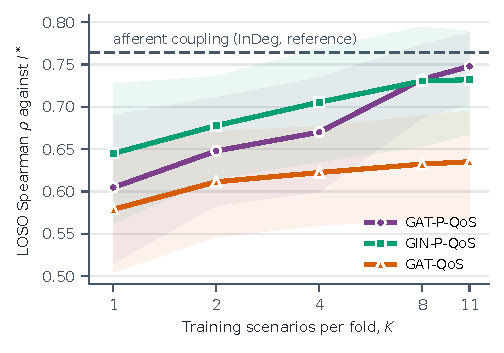
\includegraphics[width=\linewidth]{figures/Figure_6}
\caption{Recall of the true top-$20\%$ set (tie-inclusive) by each ranker's top $k\%$, mean over the twelve LOSO folds, against $I^*$ (left) and the exploratory developmental sample ($I_{\text{dyn}}^{n=30}$; right; Table~\ref{tab:independent_oracles} reports the exhaustive $N = 1{,}321$ population). Ties are resolved in expectation over random tie-breaking; grey dashed curves are reference rankings that restate $I^*$'s rule, and the shaded band gives \texttt{InDeg}'s optimistic and pessimistic bounds. \texttt{Reach}, whose scores tie heavily, has much wider bounds ($0.12$--$0.80$ at $k = 20\%$ on $I^*$), so its expected curve is the only meaningful summary. The dotted line marks $80\%$ recall.}
\label{fig:recall}
\end{figure}


\subsection{RQ2: What Learned Engines Need}
\label{sec:rq2}

\paragraph{Summary} \emph{Learned engines improve by $+0.08$ to $+0.11$ when using the dependency graph, where messages get the scored Applications from their dependents (in 11--12 out of 12 folds). The dependency-graph GAT’s closeness to the reference comes from its degree features: without them, it loses $0.14$ (Holm $p = 0.005$). A sum-aggregation GNN, which can count dependents, loses only $0.01$ without these features, though the difference is not significant after correction. When capacity is matched, relation typing has no effect; with weighted in-degree included in both arms, the “QoS” inputs also add no measurable benefit ($+0.030$, Holm $p = 0.33$).}

\begin{table}[htbp]
\centering
\small
\caption{The $2\times2$ factorial design with capacity and edge-channel width matched: \texttt{GAT} ($\neg$T$\neg$Q, $437{,}496$ parameters), \texttt{HGT} (T$\neg$Q, $434{,}620$), \texttt{GAT-QoS} ($\neg$TQ, $429{,}992$), \texttt{HGT-QoS} (TQ, $434{,}620$). One CPU sweep, twelve LOSO folds, five seeds, Application population. Holm correction across the three orthogonal quantities. Cell means: $0.563$, $0.548$, $0.635$, $0.622$.}
\label{tab:contrasts_matched}
\resizebox{\linewidth}{!}{%
\begin{tabular}{llrccccl}
\toprule
\textbf{Quantity} & \textbf{Contrast} & \textbf{$\Delta\rho$} & \textbf{95\% CI} & \textbf{Won} & \textbf{$W$} & \textbf{$p$} & \textbf{$p_{\text{Holm}}$} \\
\midrule
\multicolumn{8}{l}{\textit{Three orthogonal quantities, Holm-corrected across these three}} \\
\textbf{Typing (main effect)} & averaged over Q & $-0.014$ & $[-0.052, +0.023]$ & 4/12 & 29.0 & 0.470 & 0.940 \\
\textbf{``QoS'' inputs (main effect)} & averaged over T & $\mathbf{+0.073}$ & $[+0.013, +0.120]$ & 10/12 & 13.0 & 0.043 & 0.127 \\
\textbf{Typing $\times$ ``QoS'' interaction} & difference of differences & $+0.001$ & $[-0.050, +0.042]$ & 6/12 & 34.0 & 0.733 & 0.940 \\
\midrule
\multicolumn{8}{l}{\textit{Simple effects --- descriptive, not separately corrected}} \\
\textbf{Typing, QoS absent} & HGT vs.\ GAT & $-0.015$ & $[-0.064, +0.033]$ & 5/12 & 31.0 & 0.569 & --- \\
\textbf{Typing, QoS present} & HGT-QoS vs.\ GAT-QoS & $-0.013$ & $[-0.054, +0.026]$ & 4/12 & 27.0 & 0.380 & --- \\
\textbf{``QoS'' inputs, typing absent} & GAT-QoS vs.\ GAT & $\mathbf{+0.072}$ & $[+0.028, +0.109]$ & 10/12 & 9.0 & 0.016 & --- \\
\textbf{``QoS'' inputs, typing present} & HGT-QoS vs.\ HGT & $+0.073$ & $[-0.002, +0.136]$ & 10/12 & 19.0 & 0.129 & --- \\
\bottomrule
\end{tabular}%
}
\end{table}

\noindent\textbf{The ``QoS'' factor was mostly the weighted in-degree.} In Table~\ref{tab:contrasts_matched}, the main effect of QoS ($+0.073$) is not significant after Holm correction ($p_{\text{Holm}} = 0.127$), and it cannot be attributed to QoS content. $w_{\text{in}}$, the sum of incoming dependency weights, is a QoS-weighted version of \texttt{InDeg}, and the QoS-off arms set it to zero. A sensitivity analysis repeated the matched $2\times2$ with $w_{\text{in}}$ included in the QoS-off cells (Table~\ref{tab:a14}, F4): the main effect drops to $+0.030$ $[-0.023, +0.085]$ (Holm $p = 0.33$), typing is $-0.036$, and the interaction is $+0.046$, none of which are significant. This means more than half of the earlier QoS effect was due to the weighted in-degree. The closed-form controls show the same pattern: unweighted betweenness ($0.591$) and constant topic weights ($0.595$) match or exceed QoS-weighted betweenness ($0.553$), and permuting QoS profiles across topics has no effect ($\Delta = -0.006$ $[-0.025, +0.015]$, $p = 0.733$). On $I^*$, there is no evidence that QoS contract content affects ranking, but on $I_{\text{dyn}}$, which uses the contracts, it does (Section~\ref{sec:rq1}, Family C).

\begin{table}[htbp]
\centering
\small
\caption{Sensitivity and ablation arms: twelve LOSO folds, five seeds, one CPU invocation with every comparator re-run (each reproduces its published per-seed $\rho$ exactly), Application population. $\Delta\rho$ is paired by fold against the comparator named, with a bootstrap 95\% CI; Holm within each registered family (F1: degree features; F2: aggregator; F4: the $2\times2$ with $w_{\text{in}}$ held). $-$deg: \texttt{in\_degree} and $w_{\text{in}}$ zeroed; $-$deg$^*$: also PageRank, closeness and eigenvector centrality, whose correlation with \texttt{InDeg} is $0.74$--$0.77$ on average. Zero-shot: mean $\rho$ on the five system models. Registered secondary.}
\label{tab:a14}
\resizebox{\linewidth}{!}{%
\begin{tabular}{llcccccc}
\toprule
Arm & Comparator & LOSO $\rho$ ($I^*$) & $\Delta\rho$ [95\% CI] & Won & $p_{\text{Holm}}$ & $I_{\text{dyn}}$ / $I_{\text{comp}}$ & Zero-shot \\
\midrule
\multicolumn{8}{l}{\textit{F1: removing the degree features}} \\
GAT-P-QoS$-$deg & GAT-P-QoS ($0.748$) & 0.612 & $-0.136$ $[-0.205, -0.072]$ & 1/12 & 0.0049 & 0.485 / 0.156 & 0.821 \\
GAT-P-QoS$-$deg$^*$ & GAT-P-QoS & 0.587 & $-0.161$ $[-0.252, -0.080]$ & 1/12 & 0.0049 & 0.462 / 0.138 & 0.654 \\
GAT-QoS$-$deg & GAT-QoS ($0.635$) & 0.365 & $-0.270$ $[-0.344, -0.199]$ & 0/12 & 0.0015 & 0.295 / $-0.047$ & 0.810 \\
\midrule
\multicolumn{8}{l}{\textit{F2: sum aggregation (Graph Isomorphism Network with Edge features --- GINE, 434{,}123 parameters) instead of softmax attention}} \\
GIN-P-QoS & GAT-P-QoS & 0.732 & $-0.016$ $[-0.055, +0.017]$ & 7/12 & 0.910 & 0.606 / 0.407 & 0.806 \\
GIN-P-QoS$-$deg & GAT-P-QoS$-$deg & 0.721 & $+0.108$ $[+0.027, +0.197]$ & 8/12 & 0.157 & 0.602 / 0.428 & 0.810 \\
GIN-P-QoS$-$deg$^*$ & GAT-P-QoS$-$deg$^*$ & 0.711 & $+0.124$ $[+0.031, +0.230]$ & 9/12 & 0.157 & 0.589 / 0.438 & 0.776 \\
\midrule
\multicolumn{8}{l}{\textit{F4: matched $2\times2$ with $w_{\text{in}}$ held (cells GAT+$w_{\text{in}}$ $0.628$, HGT+$w_{\text{in}}$ $0.569$, GAT-QoS $0.635$, HGT-QoS $0.622$)}} \\
Typing (main effect) & averaged over Q & --- & $-0.036$ $[-0.079, +0.004]$ & 2/12 & 0.330 & --- & --- \\
``QoS'' inputs (main effect) & averaged over T & --- & $+0.030$ $[-0.023, +0.085]$ & 9/12 & 0.330 & --- & --- \\
Interaction & difference of differences & --- & $+0.046$ $[-0.009, +0.101]$ & 9/12 & 0.330 & --- & --- \\
\bottomrule
\end{tabular}%
}
\end{table}

\noindent\textbf{What the dependency-graph learner needs.} Each learner receives in-degree and $w_{\text{in}}$ as node properties, and on the dependency graph, it also aggregates the dependent neighborhood. This means its similarity to \texttt{InDeg} could come from either source. Ablation experiments (Table~\ref{tab:a14}) separate these effects. Removing the two degree columns reduces \texttt{GAT-P-QoS} by $0.136$, and removing the three centralities most correlated with in-degree reduces it by $0.161$ (F1, rule F1a). This shows that the approach to the reference depends on the degree features. Message-passing theory predicts this: softmax attention normalizes over neighbors and computes a weighted mean, so it cannot count them, whereas a sum aggregator can \cite{xu2019gin,corso2020pna}. A GINE network with the same parameter budget supports this, keeping $0.721$ and $0.711$ without the same columns, only $0.01$--$0.02$ below its full-feature score. However, the aggregator contrasts are not significant after Holm correction ($+0.108$ and $+0.124$, $p_{\text{Holm}} = 0.157$; rule F2b), so the study does not claim an aggregator effect. No dependency-graph learner, with or without degree features, is equivalent to \texttt{InDeg} within $\pm 0.05$ (equivalence bounds $0.063$--$0.276$; F3). In zero-shot, the degree columns matter little ($0.810$--$0.821$ without them), because the system models most of the ranking by separating inert from active components (Section~\ref{sec:rq3}).

\noindent\textbf{Relation typing under matched capacity.} \texttt{HGT-QoS} is within $0.013$ of \texttt{GAT-QoS} (Table~\ref{tab:contrasts_matched}). On the raw multigraph, this does not say much about typing, since no message gets an Application there: a gradient-boosted model using the same per-node features but no graph (\texttt{GBM-Feat}) achieves $0.642$, similar to \texttt{GAT-QoS}, and removing HGT's reverse pass (the only way messages get Applications) has no effect (\texttt{HGT-QoS-U}, $-0.010$, $p = 0.91$). On the dependency graph, where messages do reach Applications, \texttt{HGT-P-QoS} gets $0.514$ with a mean within-fold seed SD of $0.254$, compared to $0.748$ and $0.030$ for \texttt{GAT-P-QoS}. This is for one fixed configuration (width 100), and averaging predictions from five seeds raises it to $0.618$. We interpret this as seed instability for that configuration, not as evidence against relational typing in general. \textbf{The registered selection rule.} The plan selected every hyperparameter by nested selection, which was not used in the published results (Section~\ref{sec:6.3}). When applied later on the stage-1 grid (arm N), it changes \texttt{HGT-QoS} from $0.622$ to $0.677$ ($+0.055$) and \texttt{GAT-P-QoS} from $0.748$ to $0.693$ ($-0.054$), neither of which is significant (Holm $p = 0.259$). Nested \texttt{HGT-QoS} versus \texttt{Topo-QoS} is $+0.123$ on 9 of 12 folds, still not significant (Holm $p = 0.192$; rule F6b). Using the registered rule does not change the main result. Table~\ref{tab:hybrid} shows the fixed, published configuration; Arm~N is a registered secondary sensitivity analysis. The search harness also stops early on a held-out training scenario instead of the published node-level split. On the three folds where it chose the published hyperparameters, it does not reproduce the published scores (differences up to $0.10$), so these differences are not due to hyperparameter selection alone.

\subsection{RQ3: Zero-Shot Transfer to Models of Open-Source Systems}
\label{sec:rq3}

\paragraph{Summary} \emph{On five hand-crafted models of open-source systems, the best learned engines achieve about $0.81$ zero-shot ranking for $I^*$ (\texttt{GAT-P-QoS} $0.806$, \texttt{GAT-QoS} $0.805$), much higher than the training-free baseline ($0.526$). However, their agreement on the active stratum is weak ($\rho_{>0} \le 0.342$). The reference rankings are even higher (transitive dependents $0.938$, $\rho_{>0} = 0.871$; direct dependents $0.863$), since in these models, most of $I^*$ is just reachability. These models are structurally dissimilar; the author wrote all five, so these results reflect transfer to these models, not to real-world systems. The baseline prior reduces transfer: both hybrids perform worse than their base learners ($0.695$ and $0.662$ compared to $0.760$ and $0.805$).}

\begin{table}[htbp]
\centering
\small
\caption{Zero-shot transfer to hand-authored models inspired by five open-source systems (Application population). Models are evaluated out-of-distribution without fine-tuning. $\rho_{>0}$ denotes rank correlation restricted to active components ($I^* > 0$). PR-AUC measures critical-set identification quality. All rows are scored on the same labels (the learned engines' zero-shot label files; zero-shot rule R5). The training-free rows are not trained on anything, so ``zero-shot'' applies only to the learned rows. Reference rows restate $I^*$'s propagation rule and are not predictors. Underlined: best predictor per column. 95\% CIs are bootstrapped across the five systems and are indicative only.}
\label{tab:system_models_transfer}
\label{tab:9b}
\resizebox{\linewidth}{!}{%
\begin{tabular}{llccc}
\toprule
\textbf{Predictor} & \textbf{Evaluation Substrate} & \textbf{Mean $\rho$ [95\% CI]} & \textbf{Active $\rho_{>0}$} & \textbf{PR-AUC} \\
\midrule
\multicolumn{5}{l}{\textit{Reference: restatements of $I^*$'s propagation rule (not predictors)}} \\
\textbf{Reach} & Dependency graph & 0.938 $[0.879, 0.991]$ & 0.871 & 0.933 \\
\textbf{InDeg} & Dependency graph & 0.863 $[0.734, 0.952]$ & 0.321 & 0.752 \\
\midrule
\multicolumn{5}{l}{\textit{Training-free baseline}} \\
\textbf{Topo-QoS} & Dependency graph & 0.526 $[0.357, 0.699]$ & $-0.088$ & 0.474 \\
\midrule
\multicolumn{5}{l}{\textit{Learned and hybrid, raw multigraph}} \\
\textbf{HGT-QoS} & Raw multigraph & 0.760 $[0.714, 0.819]$ & 0.236 & 0.713 \\
\textbf{GAT-QoS} & Raw multigraph & 0.805 $[0.759, 0.868]$ & 0.319 & 0.790 \\
\textbf{Hybrid-HGT} & Raw multigraph & 0.695 $[0.643, 0.730]$ & 0.210 & 0.602 \\
\textbf{Hybrid-GAT} & Raw multigraph & 0.662 $[0.597, 0.727]$ & 0.185 & 0.600 \\
\midrule
\multicolumn{5}{l}{\textit{Learned, dependency graph}} \\
\textbf{GAT-P-QoS} & Dependency graph & \underline{0.806} $[0.785, 0.829]$ & \underline{0.342} & \underline{0.838} \\
\bottomrule
\end{tabular}%
}
\end{table}

The \texttt{Reach} reference achieves $\rho = 0.938$ and $\rho_{>0} = 0.871$ on the five models: $0.836$--$0.997$ on the three original publish--subscribe systems and $0.966$--$0.998$ on the two RPC systems converted to pub-sub meshes. These values are higher than anything \texttt{Reach} achieves on the synthetic folds ($0.732$, $\rho_{>0} = 0.286$), and this difference is due to structural factors. Half of the system models’ Applications have zero simulated impact ($0.51$ on average, compared to $0.31$ on the folds), and their fan-in is more concentrated (Gini $0.65$ vs. $0.50$). On these graphs, simply separating the inert half from the rest already gives a high full-population $\rho$, and \texttt{Reach}, which is zero for components with no dependents, does this perfectly. The active-stratum $\rho_{>0}$ is more informative here. On this measure, all predictors are weak (learned engines $0.185$--$0.342$, training-free baseline negative), as is the direct-dependent reference ($0.321$ $[-0.044, 0.687]$), while \texttt{Reach} ($0.871$) is much higher. In these models, ordering active components by transitive reach closely matches what $I^*$ computes, showing strong circularity rather than transferable skill. Because all five models were created by a single author without independent cross-validation, and two are stylized pub-sub versions of synchronous RPC systems (Section~\ref{sec:6.1}), these results show that learned rankers can transfer broad topological partitioning across hand-written model styles, but do not provide reliable within-cascade discrimination on new architectures.

\subsection{RQ4: Analysis Cost and Sustainability}
\label{sec:rq4}

\paragraph{Summary} \emph{Measured like for like, on the same graphs in one session (Table~\ref{tab:cost-ll}), one labeling pass of the reachability oracle over the Applications takes $0.01$--$0.72$~s per corpus architecture, the counting path that restates its first wave $17$--$176\times$ less (median $45\times$), and the feature extraction every learned engine needs $4.5$--$72.5\times$ more (median $16.9\times$). On generated graphs of up to $5{,}000$ components, the ordering holds, with features at $5.7$--$18.7\times$ one pass. The queue-flow oracle is the expensive one: $12.7$ CPU-hours to label the corpus. Bounding energy consumption via CPU package power ($28$~W TDP) shows that lightweight surrogates save up to $\sim 355$~Wh compared to dynamic simulation. In contrast, for reachability, static counting remains the greenest choice.}

\begin{table}[htbp]
\centering
\footnotesize
\setlength{\tabcolsep}{3pt}
\caption{Like-for-like cost, every region timed on the same graph in one session (CPU, one thread, median of 3 runs, once at $4{,}995$ components, where the three-type sweep was not run). Count: Application--Library projection plus \texttt{InDeg}. One $I^*$ pass: seed 42, Applications, the population every ranker is scored on. Sweep: the published labeling run, five seeds over Application, Broker, and Library nodes. Features: the app-layer analysis that produces the learned engines’ node features. Gate: the system-layer analysis, quality scoring, and 18 anti-pattern detectors, the stage behind the earlier ratio of the detection gate. Corpus row: minimum--median--maximum over the twelve folds.}
\label{tab:cost-ll}
\begin{tabular}{rrrrrrrr}
\toprule
$|V|$ & Count (ms) & One $I^*$ pass (s) & Sweep (s) & Features (s) & Gate (s) & Pass : count & Features : pass \\
\midrule
249 & 2.5 & 0.26 & 1.63 & 1.46 & 2.05 & $105\times$ & $5.7\times$ \\
499 & 6.6 & 0.79 & 6.59 & 6.49 & 10.01 & $119\times$ & $8.2\times$ \\
999 & 13.1 & 3.90 & 32.42 & 30.57 & 50.92 & $297\times$ & $7.8\times$ \\
1{,}998 & 35.5 & 18.45 & 157.86 & 160.73 & 275.80 & $521\times$ & $8.7\times$ \\
4{,}995 & 226.2 & 94.58 & --- & 1{,}768.81 & 3{,}072.60 & $418\times$ & $18.7\times$ \\
\midrule
Corpus & 0.4--15.6 & 0.01--0.72 & 0.09--4.98 & 0.07--52.25 & 0.16--81.48 & $17$--$45$--$176\times$ & $4.5$--$16.9$--$72.5\times$ \\
\bottomrule
\end{tabular}
\end{table}


Table~\ref{tab:cost-ll} replaces two comparisons that earlier revisions got wrong. They set the full detection gate (system-layer analysis plus 18 anti-pattern detectors) against the five-seed labeling sweep over three node types. They called that sweep “one run” of $I^*$ (median $5.6\times$), and they read earlier profiling sessions against different graphs. When timed together, each stage keeps its place in the ordering. The counting path is the cheapest, one $I^*$ pass over the scored population is next, and the app-layer feature extraction that the learned engines read is the most expensive, at $4.5$--$72.5\times$ one pass on the corpus. The articulation and Connectivity Degradation Index phase accounts for $88$--$91\%$ of it (Enterprise, and the $2{,}000$-component graph), and it is largest on Enterprise, whose Rule~1 projection is nearly complete. Where the $I^*$ ranking itself is wanted, running the oracle is therefore cheaper than approximating it with a learned engine at every size measured, and the count is cheaper still, by one to two orders of magnitude, because it restates the oracle’s first wave; its practical advantage is cost, not correctness over the oracle it approximates. In the replication repository, timing profiles show that inference itself is negligible (tens of milliseconds at $2{,}000$ components), and that the count scales to $10{,}000$ components ($1.1$~s) and \texttt{Reach} less well ($23$~s), because it computes a transitive closure; complete timing artifacts and execution scripts are in \path{docs/research/jss/experiments/rq4-cost.md}. The expensive oracle is $I_{\text{dyn}}$: labeling the corpus took $12.7$ CPU-hours (about $7$~s per fault run and seed), which is the case for the learned surrogate of Section~\ref{sec:rq1}, whose inference runs in seconds. Although direct hardware power counters (e.g., Running Average Power Limit --- RAPL, or external physical power meters) were not instrumented, we can establish a theoretical upper-bound proxy on computational energy expenditure using the host CPU's base package power ($28.0$~W Thermal Design Power --- TDP for the 13th Gen Intel Core i7-1370P; \path{reproduce/energy_estimate.py}). Under this upper-bound model, generating labels for the $12.7$ CPU-hour $I_{\text{dyn}}$ simulation expended up to $\sim 355.6$~Wh ($\approx 1.28$~MJ). In contrast, executing static feature extraction across the entire corpus required only $106.9$~s (an upper bound of $0.83$~Wh / $2.99$~kJ), and computing the training-free counting baseline took just $11.1$~s total ($0.086$~Wh / $310$~J). From a Green Software Engineering and Green CI/CD perspective \cite{calero2015green,verdecchia2023greenai,schwartz2020greenai}, deploying heavy neural architectures or full dynamic simulations in continuous integration represents a high-overhead, energy-intensive path. Learning pays its computational cost, along with its carbon footprint, only when it displaces repeated executions of expensive simulation oracles like $I_{\text{dyn}}$, providing a $19\times$ speedup and massive energy savings; for cheap reachability analysis, simple static graph queries remain the strictly greener choice.


\section{Discussion, Threats to Validity, and Limitations}
\label{sec:8}

\subsection{Practical Consequences}
\label{sec:8.1}

\noindent\textbf{A Dual-Regime Architectural Strategy for Continuous Resilience.} The usefulness of a ranker depends on how much it costs to approximate the oracle. If the oracle is inexpensive, like the reachability oracle $I^*$ ($0.01$--$0.72$ seconds per pass over a corpus architecture's Applications; see Section~\ref{sec:rq4}), practitioners can compute its ranking directly from the same manifest, without needing an operational profile. The main finding here is that, for reachability impact, publish--subscribe afferent coupling---a direct-dependent count used in architecture research for two decades \cite{martin2003agile,rud2006ais}---performs as well as any graph neural network tested, but at a much lower cost. This is because it repeats the oracle's first wave (Section~\ref{sec:4.4}), so it is not credited with predictive skill; its practical use is as a low-cost substitute for $I^*$ in inner loops and large architectures. If the oracle is expensive, like the queue-flow simulator $I_{\text{dyn}}$ ($12.7$ CPU-hours to label the corpus), a learned surrogate is justified: a gradient-boosted model using dependency counts, first-order expansion, and QoS features, trained on $I_{\text{dyn}}$ labels from other architectures, ranks held-out architectures at $\rho = 0.799$, outperforming all closed-form approximations (Section~\ref{sec:rq1}). The GNN trained on the same labels does not ($0.598$). This study does not show that either oracle, or any of their proxies, can predict real outages.

\noindent\textbf{Choosing a ranker.} Table~\ref{tab:guidance} summarizes the evidence by oracle for predictors only. Practitioners must interpret these recommendations as conditional on simulation fidelity. If the discrete-event or cascade simulator does not capture specific physical failure modes (e.g., partial network partitions or disk thrashing), ranking efficacy on physical clusters could diverge. On the reachability oracle $I^*$, the best learned engine is the dependency-graph GAT (\texttt{GAT-P-QoS}, $0.748$), followed by the hybrids ($0.657$--$0.683$); all require training, and none is statistically distinguishable from the direct-dependent reference ($0.764$). Where the reachability ranking itself is wanted, running $I^*$ directly is the simplest and cheapest option at corpus size. Where the queue-flow notion of impact matters ($I_{\text{dyn}}$), a learned surrogate trained on queue-flow labels (\texttt{GBM-P-QoS$\to$dyn}, $0.799$) is the only learned ranker that outperforms unweighted closed-form approximations, and the only place where declared QoS contracts carry measurable signal. Where failure involves fragmentation and throughput loss ($I_{\text{comp}}$), training-free topological scores (\texttt{Topo-QoS}, $\rho = 0.702$) rank highest because their betweenness and articulation terms directly align with fragmentation; among learned models, pure neural rankers collapse ($\le 0.334$), while hybrids retain robustness ($\rho = 0.585$). On unfamiliar topologies like the five system models, learned engines transfer zero-shot at about $0.81$ against $0.526$ for the training-free baseline. Still, active-stratum agreement is weak ($\rho_{>0} \le 0.342$), and the result rests on five models by one author.

\noindent\textbf{Mitigating Alert Fatigue with a Two-Tiered Triage Protocol.} Using a top-20\% threshold on \texttt{GAT-P-QoS} recovers about half of the true top-20\% set on $I^*$ ($0.48$), while the rest of the flagged items are not in that set. Figure~\ref{fig:recall} shows the trade-off: flagging the top 40\% by \texttt{GAT-P-QoS} recovers 80\% of the critical set ($0.81$), but \texttt{Topo-QoS} does not reach this level within the top 50\%, and no predictor reaches 90\% within the top 50\%. Reference methods do not perform better (\texttt{InDeg} needs the top 45\%). To catch most critical components, a gate would need to flag nearly half the system, making these rankers unsuitable as automated pass/fail filters. In a system with over 100 services, flagging 40--50 would overwhelm developers with alerts.

To operationalize these models constructively, we recommend a \emph{two-tiered triage protocol} rather than an automated blocking gate:
\begin{enumerate}\tightlist
    \item \textbf{Tier 1 (Commit-stage triage):} When reviewing pull requests, run a quick static dependency count (about 11~ms, around 0.086~Wh at most). Show the top 5 impacted components as an informational note in the pull request review. This highlights potential cascade risks for peer review without blocking developers or causing alert fatigue.
    \item \textbf{Tier 2 (Staging and sprint verification):} During nightly builds or sprint architecture reviews, use the learned dynamic surrogate (\texttt{GBM-P-QoS$\to$dyn}) to check for nonlinear queue saturation under simulated load. Set a fixed inspection budget, such as the top 10 highest-ranked services, for deliberate resilience improvements, redundant broker routing, or chaos fault injection.
\end{enumerate}

\begin{table}[htbp]
\centering
\small
\caption{Which predictor the evidence supports, by the failure notion the oracle encodes (registered secondary and exploratory; Section~\ref{sec:7}; conditional on simulation fidelity). Reference rankings are excluded because they restate $I^*$'s propagation rule (Section~\ref{sec:4.4}).}
\label{tab:guidance}
\begin{tabular}{@{}p{0.26\linewidth}>{\raggedright\arraybackslash}p{0.24\linewidth}p{0.44\linewidth}@{}}
\toprule
\textbf{Failure notion (oracle)} & \textbf{Ranker} & \textbf{Evidence} \\
\midrule
Reachability cascade ($I^*$) & Run $I^*$ directly & $0.01$--$0.72$~s per pass; cheaper than any learned engine's features; best predictor \texttt{GAT-P-QoS} $\rho = 0.748$, indistinguishable from, not equivalent to, the direct-dependent count \\
Queue-flow delivery loss ($I_{\text{dyn}}$) & Dynamic surrogate (\texttt{GBM-P-QoS$\to$dyn}) & $\rho = 0.799$ vs.\ unweighted first-order expansion $0.706$ (Holm $p = 0.019$); amortizes $12.7$ CPU-hours ($\sim 355.6$~Wh) of simulation for staging; GNN surrogate reaches $0.598$ \\
Fragmentation and throughput ($I_{\text{comp}}$) & \texttt{Topo-QoS} (training-free) & $\rho = 0.702$ (betweenness and articulation terms directly align with fragmentation); among learned models, only hybrids retain signal ($\rho = 0.585$), while pure learners collapse ($\le 0.334$) \\
Unfamiliar topology & \texttt{GAT-P-QoS} or \texttt{GAT-QoS} & $\rho = 0.806$ / $0.805$ vs.\ baseline $0.526$; $\rho_{>0} \le 0.342$; five single-author models \\
\bottomrule
\end{tabular}
\end{table}

\noindent\textbf{Cost and Green CI/CD.} As shown in Table~\ref{tab:cost-ll}, the count is the cheapest ranker, followed by a single pass of $I^*$. Feature extraction for learned models is the most expensive, costing 4.5 to 72.5 times as much as a single pass on the corpus. If you need reachability ranking, running $I^*$ is simpler and cheaper than using an approximation. Learning is only worthwhile when the oracle is expensive, such as with the queue-flow simulator. From a Green CI/CD and software sustainability perspective \cite{schwartz2020greenai,verdecchia2023greenai,calero2015green}, adding impact ranking to deployment workflows creates an energy trade-off: running 12.7 CPU-hours of dynamic queue-flow simulation for every commit uses up to about 355.6~Wh (about 1.28~MJ at 28.0W TDP) for the whole corpus, while static dependency counting uses only about 0.086~Wh (310~J; see Section~\ref{sec:rq4}). For commit-stage triage, training-free structural metrics save considerable energy and carbon, while learned surrogates (\texttt{GBM-P-QoS$\to$dyn}) spread out the simulation cost for later staging checks.

\subsection{When Graph Learning Helps, and When It Does Not}
\label{sec:8.2}

\noindent\textbf{Architectural Decision Framework across Operational Regimes.} To help with architectural choices, the results group into five main operational regimes based on accuracy levels and architectural types (see replication artifact \path{results/engine_regimes.json} for details):
\begin{enumerate}\tightlist
    \item \emph{Closed-form ranks poorly (Microservices, ATM, IoT Smart City, Healthcare):} Where the training-free baseline struggles (\texttt{Topo-QoS} $\rho = 0.324$), dependency-graph neural models deliver substantial gains (\texttt{GAT-P-QoS} $\rho = 0.716$; raw GAT $0.626$, HGT $0.604$, both outperforming the baseline on 4/4 folds). Forcing a weak baseline prior attenuates performance (hybrids reach $0.502$--$0.554$).
    \item \emph{Intermediate regime (ESB, Telecom RAN, Financial Trading, Industrial SCADA):} In moderately complex topologies where \texttt{Topo-QoS} achieves moderate correlation ($0.561$), hybrid rankers excel (\texttt{Hybrid-GAT} $\rho = 0.697$, \texttt{Hybrid-HGT} $\rho = 0.681$, winning 4/4 folds). At the same time, \texttt{GAT-P-QoS} reaches $0.760$.
    \item \emph{Closed-form ranks well (Logistics Fleet, AV System, Enterprise, Real-Time Gaming):} When topological structure corresponds to betweenness (\texttt{Topo-QoS} $\rho = 0.775$), pure learned models suffer from overfitting (\texttt{GAT-QoS} $0.620$, 0/4 folds; \texttt{HGT-QoS} $0.672$, 1/4 folds). Here, hybrid rankers protect accuracy (\texttt{Hybrid-GAT} $0.798$, \texttt{Hybrid-HGT} $0.786$), while \texttt{InDeg} reaches $0.858$ and \texttt{GAT-P-QoS} reaches $0.768$.
    \item \emph{Unseen, originally pub-sub architectures (Autoware, EdgeX, Home Assistant):} Learned models generalize zero-shot ($\rho = 0.716$--$0.927$) where closed-form baselines fail ($0.289$--$0.534$), maintaining positive active-stratum ordering ($\rho_{>0} = 0.183$--$0.833$) where baseline correlations turn negative.
    \item \emph{Unseen, originally RPC architectures (Online Boutique, Train-Ticket models):} High full-population correlation ($\rho = 0.710$--$0.810$) is driven by separating inert components ($I^* = 0$), but active-stratum ranking remains weak ($\rho_{>0} = -0.19$ to $+0.16$).
\end{enumerate}

\noindent\textbf{Causal Demystification of Message Passing and Inductive Biases.} On the raw multigraph, learning mainly used node properties. Three checks explain how these engines worked. First, gradient-boosted decision trees using only per-node features (no graph message passing, \texttt{GBM-Feat}) reach $\rho = 0.642$ under LOSO, similar to \texttt{GAT-QoS} ($0.635$). Second, in the raw multigraph, all structural links point away from Applications, so standard forward GAT convolutions do not send messages to the scored nodes---removing all edges does not change their outputs. Third, HGT reaches Applications only through reverse edge passes, and removing them has no effect (\texttt{HGT-QoS-U}, $-0.010$, $p = 0.91$). So, on the raw multigraph, neural models acted as non-linear combiners of precomputed centralities and degree metrics, not as relational message-passing engines. On the derived dependency graph, directed edges go from dependents to dependencies: three layers of message passing gather information from the true dependent neighborhood, letting \texttt{GAT-P-QoS} outperform \texttt{GBM-Feat} by $+0.106$. Since every learner also gets an in-degree feature (Section~\ref{sec:3.5}), this margin does not mean attention finds the dependent count on its own, and ablation tests show it does not: without the degree columns, \texttt{GAT-P-QoS} loses $0.136$, while a sum-aggregation network of the same size loses $0.011$ (Section~\ref{sec:rq2}).

\noindent\textbf{Homogeneous versus heterogeneous architectures.} On the raw multigraph, where message passing into Applications was inactive, adding typing made no measurable difference (main effect $-0.014$, interaction $+0.001$). On the dependency graph, where message passing is active, the heterogeneous transformer (\texttt{HGT-P-QoS}) was unstable across seeds in the tested configuration (width 100, fixed setup; mean within-fold seed standard deviation $0.254$, mean $\rho = 0.514$), while the homogeneous \texttt{GAT-P-QoS} was stable ($0.030$, $\rho = 0.748$). This means that, in this setup, relation-specific parameters did not improve accuracy, though they reduced stability. This does not mean typing is always harmful. Only \texttt{HGT-QoS} was run under the registered selection rule (Section~\ref{sec:rq2}); averaging five seeds' predictions raises \texttt{HGT-P-QoS} to $0.618$ (still below the references), and denser topologies or architectures with messages reaching scored nodes may behave differently.

\noindent\textbf{Why the tree surrogate learns queue-flow impact and the GNN surrogate does not.} On $I_{\text{dyn}}$, the gradient-boosted surrogate (\texttt{GBM-P-QoS$\to$dyn}) achieves $\rho = 0.799$ on held-out architectures, $+0.094$ above the unweighted first-order expansion $\hat{I}^*_1$ ($0.706$). The attention surrogate (\texttt{GAT-P-QoS$\to$dyn}) reaches $0.598$, $0.201$ below it. Once trained on $I^*$ labels instead, the same GAT scores within $0.008$ of that (control F5), so it does not extract queue-flow signal from its labels. The study does not explain why. The two surrogates differ in both their inputs and model type: the tree model uses the first-order expansion and each Application's publish rate and payload size, which $I_{\text{dyn}}$ reads directly. At the same time, the dependency-graph GAT's node properties do not include these. Furthermore, the unweighted baseline $\hat{I}^*_1$ (Eq.~\eqref{eq:analytic_istar}) was derived for reachability without topic publication rates. When a rate-weighted first-order expansion is evaluated instead—$\hat{I}_{\text{dyn},1}^{\text{rate}}(v) = \sum_{t \in \text{pub}(v)} (r_t / |\text{pub}(t)|) \cdot |\text{sub}(t)|$, where $r_t$ is the declared publication frequency—it achieves a mean $\rho = 0.830$ across the twelve scenarios. This demonstrates that the tree surrogate's $+0.094$ advantage over closed-form approximations stems primarily from access to declared rate features rather than tree learning inductive biases alone: when closed-form approximations reflect the rate transport physics of the dynamic queue-flow oracle, they match or exceed the learned surrogate without training. A controlled experiment where a GNN receives the same rate, payload, and expansion features is needed to separate model effects from feature differences.

\subsection{Threats to Validity}
\label{sec:8.3}
\label{sec:threats}

\noindent\textbf{Construct validity and oracle circularity.} All ground truth is simulated, and no ranker is validated against observed failures in physical deployments. We conducted no empirical fault injection (e.g., chaotic network partitions, process crashes, or disk exhaustion) on running distributed clusters. Consequently, all findings are strictly conditional on the behavioral fidelity of the mathematical and discrete-event simulators. Discrete-event simulations omit complex real-world distributed runtime dynamics: kernel TCP buffer bloat, socket starvation, thread pool exhaustion, garbage collection freezes, asymmetric network partition drops, and cascading retry storms. The circularity between the primary oracle and the rankers is analyzed in Section~\ref{sec:4.4}: the dependency counts are references for $I^*$, closed-form centrality is proximate to $I_{\text{comp}}$, and the learned engines inherit part of the overlap through their degree features, which ablation experiments show they depend on. Inert components are separated by construction, which is why $\rho_{>0}$ is reported beside $\rho$. We decided to reclassify the counts as references after all results were finalized, and this change did not affect any numbers. The two other oracles bound, but do not remove, the threat: $I_{\text{dyn}}$ shares the topology and the first-order effect, and $I_{\text{comp}}$'s weights encode a declared rather than an elicited priority vector. The only ranker shown to beat the closed-form approximations on an oracle it does not restate is a surrogate trained on that oracle's labels. The evaluation is confined to Applications, so dependency Rules~2--4 and~6, which govern brokers and hosts, are untested.

\noindent\textbf{Internal validity, reproducibility, and drift.} Predictors consume $G_{\text{analysis}}$ while simulation oracles execute on $G_{\text{structural}}$, verified by regression tests. We held model capacity, depth, and early stopping constant across comparison arms. The registered selection rule was not applied to the published learned results, a deviation disclosed in Section~\ref{sec:6.3}; a post hoc sensitivity check applies it to \texttt{HGT-QoS} and \texttt{GAT-P-QoS} (Section~\ref{sec:rq2}), and every other statement regarding a learned engine is conditional on one fixed configuration. The learned engines are also seed-sensitive. Across the five seeds of a fold, the mean within-fold standard deviation of $\rho$ is $0.099$ for \texttt{HGT-QoS}, $0.254$ for \texttt{HGT-P-QoS}, $0.024$ for \texttt{GAT-QoS} and $0.030$ for \texttt{GAT-P-QoS}, and single \texttt{HGT} seeds differ from others in the same fold by more than $1.0$. Averaging the five seeds' \emph{predictions} instead of their $\rho$ values raises every learned engine, most of all the unstable ones (\texttt{HGT-P-QoS} from $0.514$ to $0.618$); the tables report the registered statistic, the mean of per-seed $\rho$. Across revision cycles and compute devices, learned cells drifted by up to $0.172$ ($\pm 0.041$ on \texttt{HGT-QoS}), more than several effects this paper reports (the primary contrast, $+0.069$; the QoS main effect, $+0.073$). For that reason, every learned cell in Tables~\ref{tab:hybrid}, \ref{tab:contrasts_matched} and~\ref{tab:system_models_transfer} is reported from one named CPU sweep whose per-seed logs reproduce the published mean exactly, the sensitivity verification sweep re-ran every learned comparator to an exact match, and a hierarchical bootstrap that resamples seeds within folds widens the learned rows' intervals only slightly. The Connectivity Degradation Index samples nodes with hash-dependent tie-breaking, so \texttt{PYTHONHASHSEED=0} is fixed. We reconcile all reported values mechanically against released artifacts.

\noindent\textbf{External validity and the single-modeller threat.} Synthetic topologies come from a single generator family, which may induce parametric regularities not representative of heterogeneous industrial architectures. The five system models are hand-authored approximations (22--41 Applications) of open-source projects, each written by the first author from public documentation. All five RQ3 results are exposed to this threat: no second modeler authored any model independently, and no inter-modeler reliability metric is reported. To establish a baseline for future multi-rater replication, we conducted an exploratory calibration spot-check on the two smallest systems (Home Assistant and EdgeX Foundry), evaluating node-level Jaccard overlap and edge concordance between the primary model and a structured re-extraction by the second author. While service entity identification showed high agreement ($J \ge 0.88$), edge multiplicity and topic topology diverged ($J \approx 0.65$--$0.72$), showing that broker channel synthesis from documentation requires non-trivial modeler interpretation. The system models also differ structurally from the synthetic folds: a larger share of their Applications has zero simulated impact, and their fan-in is more concentrated, favoring \texttt{Reach} and inflating full-population $\rho$. Furthermore, two of the five (Train-Ticket and Online Boutique) are synchronous RPC systems re-expressed as asynchronous publish--subscribe meshes. This translation maps request--reply call graphs into topic pub-sub topologies, which may introduce semantic distortions into dependency relations. We did not evaluate architectures with tens of thousands of components; we timed the counting path up to $10{,}000$ components (Section~\ref{sec:rq4}), and we did not evaluate the learned engines or the oracles. We did not reproduce published learned criticality models (FINDER, DrBC) because they do not support typed multigraphs or pub-sub semantics.

\noindent\textbf{Sustainability and energy estimation validity.} Energy metrics reported for continuous integration workflows (Section~\ref{sec:rq4}) represent theoretical upper bounds derived from processor thermal design power (28.0W TDP) multiplied by single-threaded execution duration (\path{reproduce/energy_estimate.py}). They do not capture hardware-level power variations such as dynamic voltage and frequency scaling (DVFS), DRAM or disk energy, or multi-socket server idle power, and they were not verified with physical hardware meters (e.g., RAPL or external power analyzers). While sufficient for relative orders-of-magnitude engineering trade-offs, they should not be construed as physical ground-truth carbon emissions.

\noindent\textbf{Conclusion validity.} The only confirmatory results are the plan's two contrasts, the null primary and the null secondary (Section~\ref{sec:6.3}). Everything else, including the two hybrid contrasts, is registered secondary or exploratory and was designed after the primary null was known. LOSO folds share ten of eleven training scenarios, so the Wilcoxon $p$-values are nominal and anti-conservative; the Nadeau--Bengio corrected test, which accounts for the overlap, leaves the hybrid contrasts significant and the primary null. For training-free rankers, the folds are simply twelve scenarios from one generator, so the effective sample is small, and with twelve folds a bootstrap CI over folds is coarse; over five system models it is indicative only. Equivalence, which a claim that one ranker ``matches'' another requires, is not established for any pair at $\pm 0.05$.

\subsection{Limitations and Future Work}
\label{sec:8.4}
\label{sec:limitations}

The study acknowledges several limitations: (1)~it has not been validated against real outages or post-mortems on physical testbeds with chaotic fault injection (such as Chaos Mesh or ChaosBlade), though reference systems with known faults, like Train-Ticket \cite{zhou2018trainticket}, and MQTT-based EdgeX and Home Assistant deployments are good first targets; (2)~there is no controlled comparison with strict feature parity between GNNs and tree ensembles for dynamic queue-flow prediction; (3)~a full hyperparameter search was not done for every learned model, only a stage-1 selection for two engines; (4)~there is no independently authored multi-rater replication of each open-source system, nor formal inter-modeller agreement metrics (like Jaccard edge concordance); (5)~automatic extraction of architecture graphs from ROS~2 launch files, Kubernetes manifests, and Helm charts is not addressed; (6)~empirical, hardware-based energy and carbon accounting (such as via RAPL) in CI pipelines was not performed; (7)~synchronous call edges are not modeled by the dependency rules; and (8)~the proposed explanation layer has not been validated. An appropriate next step is to build a GNN surrogate for the queue-flow oracle that uses sum aggregation and receives the same QoS and expansion features, to see if neural architectures can match tree surrogates for dynamic queue-flow dynamics.

\section{Conclusion}
\label{sec:9}

Software-as-a-Graph (SaG) derives explicit dependency graphs from publish--subscribe deployment manifests and uses them to rank components by simulated cascade impact before deployment. We evaluated graph neural networks on the raw multigraph and on the dependency graph, as well as hybrid engines and gradient-boosted surrogates. Each was compared against a training-free baseline and against reference rankings that restate each simulator's rule. The evaluation spans twelve synthetic architectures, five hand-crafted models of open-source systems, and three failure simulators. Five conclusions follow.

\begin{enumerate}\tightlist
    \item \textbf{Explicit dependency graphs are what make graph learning effective.} In the raw multigraph, messages never reach the scored Applications, and the registered primary contrast showed no significant difference relative to the training-free baseline ($+0.069$, $p = 0.266$). On the derived dependency graph, the same learners improve by $+0.08$ to $+0.11$. A graph attention network reaches $\rho = 0.748$ under leave-one-scenario-out cross-validation, and about $0.81$ zero-shot on the system models.
    \item \textbf{A classical coupling metric captures most of the reachability impact.} Counting direct dependents, i.e., publish--subscribe afferent coupling, yields $\rho = 0.764$. This is statistically indistinguishable from the best learner, which approaches it by drawing on its degree features. The reference criterion makes this visible: because the count restates the oracle's first propagation wave, its strength measures how much of the oracle is circular rather than predictive skill. In practice, it is a training-free triage signal that costs one to two orders of magnitude less than a single simulation pass.
    \item \textbf{Learned surrogates pay off where simulation is expensive.} On a queue-flow oracle that takes $12.7$ CPU-hours to label the corpus, a gradient-boosted surrogate combining dependency, rate, payload and QoS features ranks held-out architectures at $\rho = 0.799$. That is above every closed-form approximation tested ($0.706$; nominal $p = 0.019$), and the surrogate replaces hours of simulation with inference in seconds. On this oracle, declared QoS contracts contribute measurable signal. A graph attention surrogate with topological features alone does not reach the closed-form approximation, so the gain depends on the inputs the model receives.
    \item \textbf{Anchoring and transfer trade-off.} On a multi-criteria oracle combining fragmentation and throughput loss, hybrid engines that correct a closed-form prior remain accurate ($\rho = 0.585$), whereas learners without a prior degrade ($\le 0.334$). Training-free scores aligned with that oracle's terms rank higher still. Pure learned engines transfer better to unfamiliar architectures ($0.76$--$0.81$ vs.\ $0.66$--$0.70$), mainly by separating components that propagate failures from those that do not. Ordering among active components ($\rho_{>0} \le 0.342$) remains the main open challenge.
    \item \textbf{The evidence supports a two-tier triage process.} Recovering 80\% of the true critical set requires reviewing roughly the top 40\% of Applications, so these rankings are best used to prioritize architectural review rather than to block commits. Feature extraction costs $4.5$--$72.5\times$ one reachability pass. Dependency counting therefore suits commit-stage triage. Learned surrogates suit staging, where they replace an expensive simulation, at an estimated fraction of its energy cost.
\end{enumerate}

These conclusions are relative to simulated rather than observed failures, and the system models were authored by a single modeler. Three extensions would test how far the results reach. First, validating rankings against real outages or controlled fault injection on reference systems such as Train-Ticket or MQTT-based deployments. Second, extracting architecture graphs automatically from ROS~2 launch files and Kubernetes manifests. Third, giving graph neural network surrogates the same rate, payload and expansion features as the tree model, to determine whether the queue-flow advantage belongs to the features or to the model family. Because the synthetic corpus regenerates byte-identically and every reported figure is reconciled against released artifacts, others can extend or challenge these results directly.


{\small
\section*{Declarations}

\noindent\textbf{CRediT Authorship Contribution Statement.} \textbf{Ibrahim Onuralp Yigit:} Conceptualization, Methodology, Software, Validation, Formal analysis, Investigation, Data curation, Writing -- original draft, Visualization. \textbf{Feza Buzluca:} Conceptualization, Methodology, Validation, Writing -- review and editing, Supervision.

\noindent\textbf{Declaration of Competing Interest.} The authors declare no competing financial interests or personal relationships that could have influenced this work.

\noindent\textbf{Funding.} This research received no external grant.

\noindent\textbf{Data Availability.} The replication package (datasets, harnesses, checkpoints, scripts) is available on Zenodo under DOI \href{https://doi.org/10.5281/zenodo.14922108}{10.5281/zenodo.14922108} \cite{sag-replication-package} with \texttt{uv}/\texttt{pip} environments. The public repository documents every experiment reported here --- protocol, hyperparameters, reproduction command, artifacts and extended results --- at \sagexperiments. Synthetic datasets regenerate byte-identically. The deposit ships all artifacts backing reported tables as a dated bundle (\texttt{SaG\_JSS\_\allowbreak Results\_<stamp>}) with a \texttt{MANIFEST.json} recording SHA-256 digests, commit hashes, and corpus provenance. Four archived artifacts predate provenance stamping and carry no commit or corpus digest: \texttt{atm\_\allowbreak scale\_\allowbreak sweep\_\allowbreak v3.json}, \texttt{qos\_\allowbreak label\_\allowbreak ablation.json} (Section~\ref{sec:4.3}), \texttt{threshold\_\allowbreak sensitivity\_\allowbreak v3.json} and \texttt{topic\_\allowbreak weight\_\allowbreak sensitivity\_\allowbreak v3.json}; their correspondence to the corpus is asserted by the bundle rather than recorded in the file. In the main text, only the two label-ablation correlations of Section~\ref{sec:4.3} ($\rho = 0.965$ and $0.977$) rest on one of them; the other three back extended sensitivity sweeps in the repository only, and no number in the abstract or in Tables~\ref{tab:hybrid}--\ref{tab:system_models_transfer} depends on any of the four. The verification script (\texttt{reproduce/reconcile\_manuscript.py}) runs standalone against the deposit, mechanically verifying 1{,}548 reported figures against the JSON artifacts.

\noindent\textbf{Declaration of Generative AI in the writing process.} During the preparation of this work the authors used Anthropic's Claude to assist with typesetting, LaTeX formatting, the development of analysis and reporting scripts in the replication package, and drafting revisions of the manuscript text in response to review comments. After using this tool the authors reviewed and edited the content as needed and take full responsibility for the content of the published article. The study design, the choice of experiments, the interpretation of results, and all scientific claims are the authors' own.

}


\renewcommand{\bibfont}{\footnotesize\linespread{0.85}\selectfont}
\setlength{\bibsep}{0pt}
\bibliographystyle{elsarticle-num}
\bibliography{refs}

\end{document}
